\documentclass[recuosum=1.5cm]{iftex2024}

\usepackage{numprint}
\npthousandsep{.}
\npdecimalsign{,}

% \DeclareUnicodeCharacter{0301}{XXXXXXXXXXXXXXXXXXXXXXXXXXXX}
%\usepackage[backend=biber]{biblatex}

\usepackage{xcolor}
\usepackage{minted}
\usemintedstyle{borland}
\definecolor{LightGray}{gray}{0.95}

\usepackage{caption}
\usepackage{etoolbox}

%% Contador para códigos
%\newcounter{codigo}[chapter]
%\renewcommand{\thecodigo}{\thechapter.\arabic{codigo}}
%
%% Comando para título e label do código
%\newcommand{\codigo}[2]{%
%	\refstepcounter{codigo}%
%	\noindent\captionof*{table}{\textnormal{Código~\thecodigo{} -- #1}}\label{#2}%
%}

\addbibresource{referencias.bib}
\titulo{Análise e integração de dados do mercado financeiro brasileiro disponibilizados pela B3 e CVM}
\autor{Vinícius Tadeu Andrade Costa}
\local{Bambuí -- MG}
\data{2025-01-18}

\campus{\textit{Campus} Bambuí}
\curso{Bacharelado}{Engenharia de Computação}
\titulacao{Bacharel}

\orientador[M]{Marcos Roberto Ribeiro}
% \coorientador{Nome da Coorientador}
% \instituicaocoorientador{Instituição do Coorientador}
% \membrobanca{Fulano de Tal}{Instituição do Fulano de Tal}
% \membrobanca{Ciclano de Tal}{Instituição do Ciclano de Tal}
% \fichacatalografica{ficha.pdf}
% \assinaturas{assinaturas.pdf}

\dedicatoria{Dedico este trabalho à minha esposa e filhos, incentivadores e fontes inesgotáveis de apoio, amor e compreensão.}

\agradecimentos{Agradeço a toda à minha família, esposa, filhos, pais e minha irmã, por acreditarem em mim e pelo incentivo constante na realização deste trabalho.

Agradeço à minha orientadora, ao meu coorientador e a todos que contribuíram de alguma forma para a realização deste trabalho.}

\epigrafe{A tarefa mais importante de uma pessoa que vem ao mundo é criar algo.}{Paulo Freire}

\resumo{Este trabalho é um modelo em {\latex} utilizando a classe \iftex.
Tal classe foi desenvolvida com base no manual de normalização de trabalhos acadêmicos do IFMG e nas normas relacionadas da Associação Brasileira de Normas Técnicas.
Este modelo apresenta uma estrutura básica com exemplos de elementos pré e pós-textuais.
Maiores informações sobre como utilizar a classe podem ser encontradas no manual da classe \iftex.}
\palavraschave{\iftex. Modelo. IFMG. \latex.}

\abstract{This work is a template in {\LaTeX} using the \iftex class.
This class was developed based on the academic work standardization manual of IFMG and the related norms of the Brazilian Association of Technical Standards.
This template presents a basic structure with examples of pre and post-textual elements.
Further information on how to use the class can be found in the \iftex class manual.}
\keywords{\iftex. Template. IFMG. \latex.}

\listafiguras
\listaquadros
\listatabelas

\listasiglas{%
 \begin{itemize}[]
  \item[IFMG] -- Instituto Federal de Educação, Ciência e Tecnologia de Minas Gerais
  \item[TCC] -- Trabalho de conclusão de curso
  \item[B3] -- Brasil, Bolsa e Balcão
  \item[CVM] -- Comissão de Valores Mobiliários
  \item[DFP] -- Demonstrações Financeiras Padronizadas
  \item[ITR] -- Formulário de Informações Trimestrais
  \item[IPE] -- Periódicos e Eventuais
  \item[FRE] -- Formulário de Referência
 \end{itemize}
}

\listasimbolos{%
 \begin{itemize}[]
   \item[$\mathbb{X}$] -- Variável X
   \item[$\mathsf{I\!R}$] -- Conjunto dos números reais
 \end{itemize}
}

\begin{document}

\maketitle

\chapter{INTRODUÇÃO}

O mercado financeiro brasileiro tem passado por transformações significativas impulsionadas pelo avanço tecnológico e pela crescente demanda por soluções que automatizem a integração e a análise de dados \cite{dantas:2020:comportamento}. Esse movimento reflete a busca constante por maior eficiência e acessibilidade nas informações financeiras, fundamentais para investidores e analistas que utilizam a análise fundamentalista como base para a tomada de decisões. 

O crescimento desse interesse pode ser observado no relatório anual de 2023 da Brasil, Bolsa e Balcão (B3), que apontou um aumento de aproximadamente 15\% no número de investidores em comparação com 2022 \cite{b3:2023:relatorio}. Esse cenário reforça a necessidade de garantir o acesso simplificado e estruturado às informações financeiras das empresas, promovendo maior eficiência nas análises e decisões de mercado.

No Brasil, dois órgãos desempenham papéis centrais na disponibilização de dados do mercado de capitais: a B3 e a Comissão de Valores Mobiliários (CVM). A B3, fundada em 1890 e sediada em São Paulo, é a única bolsa de valores do país e fornece dados sobre o histórico de negociações de ativos \cite{b3:2023:investidores}. 

Já a CVM, criada em 1976, é a entidade responsável por regulamentar e supervisionar o mercado de capitais brasileiro, disponibilizando publicamente uma ampla gama de informações contábeis e financeiras das empresas listadas na bolsa \cite{cvm:2009:informacao}. Essas informações são essenciais para investidores que utilizam a análise fundamentalista, metodologia que avalia a saúde financeira e o desempenho das empresas com base em seus demonstrativos financeiros e outros indicadores econômicos.

Embora a CVM disponibilize esses dados publicamente, seu formato dificulte a manipulação por usuários sem conhecimento técnico avançado. Muitos estão em arquivos complexos que exigem processamento adicional, criando um obstáculo para investidores e analistas que necessitam de informações ágeis e acessíveis. Essa barreira técnica restringe o acesso à informação e limita a capacidade analítica de boa parte do mercado.

A necessidade de soluções mais acessíveis já foi abordada por estudos acadêmicos. \cite{deAraujo:2021:modeloDados} propõem um modelo de dados flexível para análise fundamentalista moderna, estruturando balanço patrimonial, demonstração de resultados e fluxo de caixa em um banco de dados não relacional (MongoDB). Esse tipo de abordagem reforça a importância de alternativas que simplifiquem o acesso e a análise dos dados financeiros.


Diante desse contexto, este trabalho propõe o desenvolvimento de um sistema automatizado para a integração e análise dos dados fornecidos pela CVM, facilitando seu acesso e processamento. A solução busca oferecer uma ferramenta capaz de extrair e estruturar essas informações de forma eficiente, contribuindo para a análise fundamentalista e auxiliando na tomada de decisões. Além disso, pretende otimizar o processo de análise, tornando-o mais acessível e organizado para investidores, analistas e pesquisadores. Com essa abordagem, espera-se reduzir a complexidade no manuseio dos dados e aprimorar a compreensão do mercado.

\section{Justificativa}
A B3 apresentou um crescimento significativo no volume de negócios e de capital movimentado ao longo dos anos. Em 2023, o volume total negociado na B3 alcançou R\$ 7,2 trilhões, representando um aumento de 12,6\% em relação a 2022 \cite{b3:2023:investidores}. Além disso, o montante total de dinheiro movimentado na B3 em 2023 foi de R\$ 2,4 trilhões, um aumento de 15,5\% em relação ao ano anterior \cite{b3:2023:investidores}.

Embora os dados da B3 não estejam diretamente presentes neste trabalho, seu contexto é fundamental, uma vez que ela representa o principal ambiente de negociação de ativos no Brasil. As informações que embasam os negócios realizados na B3, especialmente aquelas relacionadas às demonstrações financeiras e dados cadastrais das empresas listadas, estão disponíveis na CVM. Dessa forma, a integração dos dados da CVM serve como uma base fundamental para análises que indiretamente impactam o entendimento do mercado da B3.

Atualmente, as informações da CVM estão disponíveis em formatos específicos, fragmentados e sem integração adequada, o que dificulta o acesso e a análise automatizada dos dados. Até o momento, não foram encontrados trabalhos que promovam essa integração de forma estruturada e com disponibilização pública.

A proposta de integrar os dados da CVM visa criar uma base de dados unificada e acessível, que sirva como suporte para futuros trabalhos acadêmicos e aplicações práticas em algoritmos de análise de mercado financeiro. Com isso, espera-se facilitar o desenvolvimento de estudos e ferramentas que contribuam para uma melhor compreensão do mercado de capitais brasileiro \cite{lindman:2020:integration}

\section{Objetivos}

Este estudo tem como objetivo principal o desenvolvimento de um sistema automatizado capaz de integrar e facilitar o acesso aos dados financeiros disponibilizados publicamente pela CVM. A proposta busca contribuir com a análise fundamentalista e apoiar o processo de tomada de decisão por parte de investidores, pesquisadores e demais interessados no mercado financeiro.

Para atingir esse objetivo, são estabelecidas as seguintes metas específicas:

\begin{itemize} 
	\item analisar a estrutura dos dados públicos fornecidos pela CVM, identificando suas fontes, formatos e padrões; 
	\item propor uma modelagem lógica que permita a integração eficiente e automatizada desses dados; 
	\item projetar e implementar um sistema que realize a extração, o processamento e a disponibilização dos dados de forma acessível e estruturada. 
\end{itemize}


\section{Resultados Esperados}

Espera-se que a ferramenta desenvolvida neste trabalho integre de forma eficiente os dados financeiros públicos disponibilizados pela CVM, permitindo a criação de uma base de dados unificada, estruturada e acessível.

Essa base será construída com foco em um recorte histórico que contemple, no mínimo, o período a partir de 2019, o que proporcionará maior profundidade nas análises e permitirá identificar padrões e variações ao longo do tempo. Tal histórico é essencial para estudos mais robustos e comparativos dentro do contexto da análise fundamentalista.

Embora os dados da B3 não sejam utilizados diretamente neste trabalho, o sistema proposto pode contribuir indiretamente para análises relacionadas à bolsa de valores, uma vez que as informações integradas da CVM servem como base para decisões tomadas por investidores e instituições que atuam no ambiente da B3.

A disponibilização pública dessa base de dados tem o potencial de promover maior transparência, acessibilidade e democratização das informações financeiras no Brasil, beneficiando pesquisadores, investidores e demais interessados no mercado de capitais.


\chapter{FUNDAMENTOS TEÓRICOS}
Este capítulo apresenta os fundamentos teóricos que sustentam o desenvolvimento deste trabalho, bem como os principais estudos e iniciativas relacionadas ao tema. A Seção \ref{sec:mercado-financeiro} aborda o mercado financeiro brasileiro, com ênfase na atuação da CVM e sua função reguladora. A Seção \ref{sec:analises} discute as diferentes abordagens de análise para investimentos, com foco na análise fundamentalista. A Seção \ref{sec:computacional} descreve a modelagem dos dados e os processos de integração utilizados no projeto. Por fim, a Seção \ref{sec:estado-arte} apresenta trabalhos acadêmicos e iniciativas similares à proposta deste estudo, destacando seus principais diferenciais.

\section{Mercado financeiro} \label{sec:mercado-financeiro} % OK

O mercado financeiro é um sistema que engloba uma variedade de instituições, instrumentos e atividades relacionadas à gestão de recursos financeiros. Ele abrange diferentes segmentos, incluindo o mercado de capitais, o mercado monetário, o mercado cambial e o mercado de derivativos. O principal propósito do mercado financeiro é facilitar a alocação eficiente de recursos entre poupadores e investidores, fornecendo oportunidades de investimento e financiamento para empresas, governos e indivíduos \cite{teixeira:2019:mercado, damodaran:2012:investimentos}.

No Brasil, o mercado financeiro é composto pelos segmentos de mercado de capitais, mercado monetário, mercado de crédito, mercado de câmbio e mercado de derivativos. O mercado de capitais envolve a negociação de ações, debêntures e outros ativos mobiliários. Esse segmento é fundamental para o financiamento das empresas, permitindo que elas captem recursos por meio da emissão de títulos negociáveis no mercado financeiro \cite{reis:2021:negociacao}.

O mercado monetário é o espaço onde ocorrem operações de curto prazo entre instituições financeiras e o Banco Central. Essas operações têm como objetivo controlar a liquidez da economia e a taxa de juros, garantindo o equilíbrio do sistema financeiro \cite{deSouzaFigueiredo:2021:mercado}.

O mercado de crédito destina-se ao financiamento de empresas e pessoas físicas por meio de empréstimos e financiamentos bancários. Esse segmento é essencial para a dinamização da economia, permitindo investimentos e consumo a partir da concessão de crédito.

O mercado de câmbio é responsável pelas transações de compra e venda de moedas estrangeiras. Sua função principal é viabilizar o comércio internacional, investimentos estrangeiros e a gestão de reservas cambiais \cite{gois:2019:efeito}.

O mercado de derivativos compreende a negociação de contratos futuros, opções e \textit{swaps}, instrumentos utilizados para a gestão de riscos financeiros. Esse segmento permite que investidores e empresas se protejam contra variações adversas nos preços de ativos e taxas de juros \cite{figueiredo:2023:capacidade}.

Dentro do mercado financeiro, as ações representam uma das principais modalidades de investimento. Uma ação é uma fração do capital social de uma empresa, conferindo ao seu detentor a propriedade de uma parcela da empresa emissora. Ao adquirir ações, o investidor se torna um sócio da empresa e pode ter direito a participação nos lucros distribuídos e, em alguns casos, a voto nas assembleias de acionistas \cite{reis:2021:negociacao, gomes:2007:bolsa}.

A negociação de ações ocorre principalmente em bolsas de valores, como a B3 no Brasil, onde investidores podem comprar e vender ativos. O preço das ações é determinado pela oferta e demanda, ou seja, pela interação entre compradores e vendedores no mercado \cite{santander:2024:pregao}. Além disso, diversos fatores influenciam a valorização ou desvalorização dos papéis, como os resultados financeiros das empresas, a conjuntura econômica e eventos geopolíticos \cite{damodaran:2012:investimentos, attie:2013:bolsa}.

Duas instituições fundamentais nesse ecossistema são a B3 e a CVM. A B3 atua como principal plataforma de negociação de ativos financeiros, enquanto a CVM desempenha um papel regulador crucial, garantindo transparência e equidade no mercado de capitais \cite{cvm:2023:funcoes}.

Criada pela Lei nº 6.385/1976 \cite{brasil:1976:lei6385}, a CVM tem como principal missão proteger os investidores e garantir o funcionamento eficiente do mercado de capitais \cite{cvm:2009:informacao}. Entre suas principais atribuições estão \cite{cvm:2009:informacao, roberto:2023:papel}:

\begin{itemize}
	\item regulamentação da abertura de capital de empresas e suas obrigações com o mercado;
	\item supervisão de corretoras, bancos de investimento e outras instituições financeiras;
	\item fiscalização da negociação de ativos financeiros e combate a fraudes e manipulações de mercado;
	\item garantia da transparência e divulgação de informações pelas companhias de capital aberto.
\end{itemize}

A CVM exige que todas as empresas listadas na bolsa de valores publiquem periodicamente suas demonstrações financeiras e outros documentos essenciais, como balanços patrimoniais e informações sobre acionistas relevantes. Essa transparência fortalece a confiança dos investidores e contribui para a estabilidade e o crescimento do mercado financeiro brasileiro \cite{fgv:2024:transformacao}.

Dessa forma, a regulamentação e a supervisão do mercado financeiro brasileiro desempenham um papel essencial na proteção dos investidores e no desenvolvimento sustentável do setor \cite{figueiredo:2023:capacidade}.

Para garantir a ampla disponibilidade dessas informações, a CVM mantém uma base de dados acessível ao público por meio de seu portal eletrônico\footnote{\url{https://dados.cvm.gov.br}.}  e sistemas especializados, como o Sistema Empresas.NET e o CVMWeb. As empresas registradas são obrigadas a enviar seus documentos periodicamente, os quais são disponibilizados em diversos formatos, como PDF, XML e XBRL, permitindo tanto a consulta manual quanto a análise automatizada \cite{cvm:2009:informacao}. Essa estrutura facilita o acompanhamento do mercado por investidores, analistas e demais interessados, promovendo maior transparência e acesso à informação.

A base de dados da CVM inclui:

\begin{itemize}
	\item demonstrações financeiras padronizadas (DFPs);
	\item informes trimestrais (ITRs);
	\item relatórios de governança corporativa;
	\item documentos de ofertas públicas de ações (IPO);
	\item dados sobre fundos de investimento e gestores de ativos.
\end{itemize}

\section{Análises para investimento} \label{sec:analises}

A análise de investimentos busca avaliar oportunidades de alocação de capital, utilizando diferentes abordagens para identificar ativos com potencial de retorno \cite{liaw:2011:business}. Entre essas abordagens, destacam-se a análise técnica, a análise de sentimento, a análise quantitativa, a análise macroeconômica e a análise fundamentalista.  

A análise técnica baseia-se no estudo de padrões gráficos e estatísticos do histórico de preços dos ativos. Os analistas técnicos utilizam indicadores como médias móveis, bandas de Bollinger e índices de força relativa para identificar tendências e pontos de compra ou venda no mercado \cite{omane:2019:time}.  

A análise de sentimento considera o impacto de notícias, redes sociais e opiniões de investidores sobre os ativos financeiros. Essa abordagem busca medir o comportamento do mercado a partir da análise de textos, discursos e volumes de menções relacionadas a determinados ativos, utilizando técnicas de processamento de linguagem natural e aprendizado de máquina \cite{kearney:2014:textual}.  

A análise quantitativa utiliza modelos matemáticos e estatísticos para prever movimentos de mercado e identificar oportunidades de investimento. Esse método frequentemente emprega algoritmos computacionais, regressões estatísticas e aprendizado de máquina para encontrar correlações e padrões em grandes volumes de dados financeiros \cite{sahu:2023:overview}.  

A análise macroeconômica avalia fatores econômicos amplos, como inflação, Produto Interno Bruto (PIB), taxas de juros e política monetária. Essa abordagem busca compreender como variáveis macroeconômicas influenciam os mercados financeiros e os preços dos ativos, sendo fundamental para investidores institucionais e gestores de fundos \cite{claessens:2017:macroeconomic}.  

A análise fundamentalista foca nos fundamentos financeiros das empresas, examinando indicadores como receita, lucro, endividamento e governança corporativa. Esse método busca determinar o valor intrínseco de um ativo, comparando-o ao seu preço de mercado para identificar se está subvalorizado ou supervalorizado. No contexto deste estudo, a análise fundamentalista será o enfoque principal, dada sua relevância na avaliação detalhada do desempenho financeiro e estratégico das companhias.  


A análise fundamentalista investiga os dados financeiros e operacionais das empresas para determinar seu valor intrínseco \cite{mathew:2024:overview}. Para isso, utiliza diversos indicadores que auxiliam na avaliação do desempenho financeiro, da estrutura de capital e da liquidez da empresa. Esses indicadores podem ser agrupados em quatro categorias principais: indicadores de rentabilidade, indicadores de liquidez, indicadores de endividamento e valor intrínseco.

\subsection{Indicadores de rentabilidade}

Os indicadores de rentabilidade medem a eficiência da empresa em gerar lucros em relação a diferentes bases financeiras. Esses cálculos são amplamente utilizados em estudos financeiros e derivam da contabilidade gerencial e da análise de demonstrações financeiras \cite{kothari:2001:capital}.

O lucro por ação (LPA) indica o montante de lucro líquido atribuído a cada ação ordinária em circulação da empresa. É um indicador essencial para avaliar o desempenho das ações no mercado.  
A fórmula é dada pela Equação \eqref{eq:lpa}. Considerando um lucro líquido de R\$ 10 milhões e 2 milhões de ações em circulação, tem-se o LPA de R\$ 5,00, conforme a Equação \eqref{eq:lpa-exemplo} \cite{omane:2019:time}.

\bigskip
\begin{subequations} \noindent
\begin{minipage}[b]{0.48\linewidth}
  \begin{equation} \label{eq:lpa}
    \text{LPA} = \frac{\text{Lucro líquido}}{\text{Número de ações}}
  \end{equation}
\end{minipage}
\hfill
\begin{minipage}[b]{0.48\linewidth}
  \begin{equation} \label{eq:lpa-exemplo}
    \text{LPA} = \frac{\numprint{10000000.00}}{\numprint{2000000.00}} = \numprint{5.00}
  \end{equation}
\end{minipage}
\end{subequations}
\bigskip

O índice preço por lucro (P/L) mede quanto os investidores estão dispostos a pagar pelo lucro da empresa.  
A fórmula está na Equação \eqref{eq:pl}. Se uma ação custa R\$ \numprint{50.00} e o LPA é R\$ \numprint{5.00}, o P/L será \numprint{10.00}, indicando que os investidores estão dispostos a pagar 10 vezes o lucro anual por ação \cite{sahu:2023:overview}.

\bigskip
\begin{subequations} \noindent
\begin{minipage}[b]{0.48\linewidth}
    \begin{equation} \label{eq:pl}
        \text{P/L} = \frac{\text{Preço da ação}}{\text{LPA}}
    \end{equation}
\end{minipage}
\hfill
\begin{minipage}[b]{0.48\linewidth}
    \begin{equation} \label{eq:pl-exemplo}
        \text{P/L} = \frac{\numprint{50.00}}{\numprint{5.00}} = \numprint{10.00}
    \end{equation}
\end{minipage}
\end{subequations}
\bigskip

O \textit{dividend yield} (DY) mede a rentabilidade dos dividendos pagos em relação ao preço da ação. Se a empresa paga R\$~\numprint{2.00} de dividendos por ação e o preço da ação é R\$~\numprint{40.00}, o cálculo da Equação~\eqref{eq:dy-exemplo} resulta em um DY de \numprint{5.00}\% \cite{kearney:2014:textual}.

\bigskip
\begin{subequations} \noindent
\begin{minipage}[b]{0.48\linewidth}
    \begin{equation} \label{eq:dy}
        \text{DY} = \frac{\text{Dividendo por ação}}{\text{Preço da ação}} \times 100
    \end{equation}
\end{minipage}
\hfill
\begin{minipage}[b]{0.48\linewidth}
    \begin{equation} \label{eq:dy-exemplo}
        \text{DY} = \frac{\numprint{2.00}}{\numprint{40.00}} \times 100 = \numprint{5.00}\%
    \end{equation}
\end{minipage}
\end{subequations}
\bigskip

\subsection{Indicadores de Liquidez}

Os indicadores de liquidez avaliam a capacidade da empresa de honrar suas obrigações de curto prazo \cite{claessens:2017:macroeconomic}. A Liquidez Corrente (LC) é expressa na Equação~\eqref{eq:lc}. Se o ativo circulante é de R\$~\numprint{500000} e o passivo circulante de R\$~\numprint{250000}, a liquidez corrente é igual a \numprint{2.00}, conforme a Equação~\eqref{eq:lc-exemplo}.

\bigskip
\begin{subequations} \noindent
\begin{minipage}[b]{0.48\linewidth}
    \begin{equation} \label{eq:lc}
        \text{LC} = \frac{\text{Ativo circulante}}{\text{Passivo circulante}}
    \end{equation}
\end{minipage}
\hfill
\begin{minipage}[b]{0.48\linewidth}
    \begin{equation}\label{eq:lc-exemplo}
        \text{LC} = \frac{\numprint{500000}}{\numprint{250000}} = \numprint{2.00}
    \end{equation}
\end{minipage}
\end{subequations}
\bigskip

\subsection{Indicadores de Endividamento}

Os indicadores de endividamento mostram a dependência da empresa em relação ao capital de terceiros \cite{kothari:2001:capital}. 

Um dos principais indicadores é a dívida bruta, que representa a soma do passivo circulante e do passivo não circulante da empresa, conforme definido na Equação~\eqref{eq:db}. A Equação~\eqref{eq:db} expressa a fórmula geral da dívida bruta, que é composta pelos valores de obrigações de curto prazo (passivo circulante) e de longo prazo (passivo não circulante). Já a Equação~\eqref{eq:db-exemplo} apresenta um exemplo numérico, onde a dívida bruta totaliza R\$~\numprint{3000000}, a partir da soma de R\$~\numprint{1000000} de passivo circulante e R\$~\numprint{2000000} de passivo não circulante.

\begin{subequations}
\begin{equation} \label{eq:db}
    \text{Dívida bruta} = \text{Passivo circulante} + \text{Passivo não circulante}
\end{equation}

\begin{equation} \label{eq:db-exemplo}
    \text{Dívida bruta} = \numprint{1000000} + \numprint{2000000} = \numprint{3000000}
\end{equation}
\end{subequations}

Por exemplo, se a dívida bruta é de R\$~\numprint{3000000} e o caixa e equivalentes de caixa totalizam R\$~\numprint{500000}, a dívida líquida será de R\$~\numprint{2500000}, conforme indicado na Equação~\eqref{eq:dl-exemplo}. A Equação~\eqref{eq:dl} define a dívida líquida, que representa o valor da dívida efetiva da empresa, descontado o montante disponível em caixa ou em aplicações de liquidez imediata. Já a Equação~\eqref{eq:dl-exemplo} ilustra esse conceito com valores hipotéticos, demonstrando que, ao subtrair R\$~\numprint{500000} disponíveis em caixa de uma dívida bruta de R\$~\numprint{3000000}, obtém-se uma dívida líquida de R\$~\numprint{2500000}.

\begin{subequations}
	\begin{equation} \label{eq:dl}
		\text{Dívida líquida} = \text{Dívida bruta} - \text{Caixa e equivalentes de caixa}
	\end{equation}
	\begin{equation} \label{eq:dl-exemplo}
		\text{Dívida líquida} = \numprint{3000000} - \numprint{500000} = \numprint{2500000}
	\end{equation}
\end{subequations}

\subsection{Valor intrínseco}

O valor intrínseco é estimado pelo método de Desconto de Fluxo de Caixa (DCF), conforme a Equação~\eqref{eq:vi}. Nessa equação, \( r \) representa a taxa de desconto e \( t \) o período de tempo. Com fluxo de caixa de R\$~\numprint{1000000} e taxa de desconto de \numprint{10}\%, o valor intrínseco resulta em R\$~\numprint{909090.91}, conforme demonstrado na Equação~\eqref{eq:vi-exemplo}. Esse cálculo reflete o valor presente do fluxo de caixa futuro \cite{figueiredo:2023:capacidade}.

\begin{subequations}
	\begin{equation} \label{eq:vi}
		\text{Valor intrínseco} = \sum \frac{\text{Fluxo de caixa esperado}}{(1 + r)^t}
	\end{equation}
	
	\begin{equation} \label{eq:vi-exemplo}
		\text{Valor intrínseco} = \frac{\numprint{1000000}}{(1 + \numprint{0.10})^1} = \frac{\numprint{1000000}}{\numprint{1.10}} = \numprint{909090.91}
	\end{equation}
\end{subequations}

\section{Modelagem e integração de dados} \label{sec:computacional}

A modelagem e integração de dados são etapas fundamentais para a construção de um sistema automatizado de análise fundamentalista. Neste trabalho, essas etapas têm o propósito de estruturar, consolidar e organizar os dados disponibilizados pela CVM, garantindo sua utilização eficiente e integrada. A seguir, são apresentadas as principais abordagens empregadas na modelagem dos dados, bem como os métodos utilizados para sua integração, assegurando a consistência, acessibilidade e interoperabilidade das informações no sistema desenvolvido.

\subsection{Modelagem dos dados e estruturação lógica}

A modelagem de dados é uma etapa fundamental no desenvolvimento de sistemas que manipulam grandes volumes de informações, especialmente em contextos financeiros, onde a integridade, consistência e escalabilidade são requisitos indispensáveis \cite{elmasri:2005:sistemas}. Neste trabalho, adotou-se uma abordagem centrada na modelagem lógica, com o objetivo de estruturar uma base de dados relacional robusta, capaz de integrar e armazenar dados públicos oriundos da CVM.

A modelagem lógica traduz os requisitos identificados no domínio do problema em uma estrutura formal que define, de maneira precisa, as tabelas, os atributos, os tipos de dados e as restrições de integridade necessárias para a representação das entidades envolvidas \cite{connolly:2015:database}. Diferente da modelagem conceitual, que geralmente se utiliza de representações como o Diagrama Entidade-Relacionamento (DER), a modelagem lógica já incorpora aspectos técnicos relacionados à implementação em um Sistema de Gerenciamento de Banco de Dados (SGBD), neste caso, o MySQL.

A Figura \ref{fig:esquema_logico} apresenta o esquema lógico elaborado com base em práticas de engenharia reversa e análise das documentações e estruturas disponibilizadas pela CVM. Essa técnica permite extrair o modelo de dados a partir de fontes existentes, facilitando o redesenho e a normalização da base de dados \cite{scannapieco:2006:data}.

\begin{figure}[!htb] 
	\centering
	\caption{Esquema lógico do banco de dados para integração de dados da CVM.} 
	\label{fig:esquema_logico}
	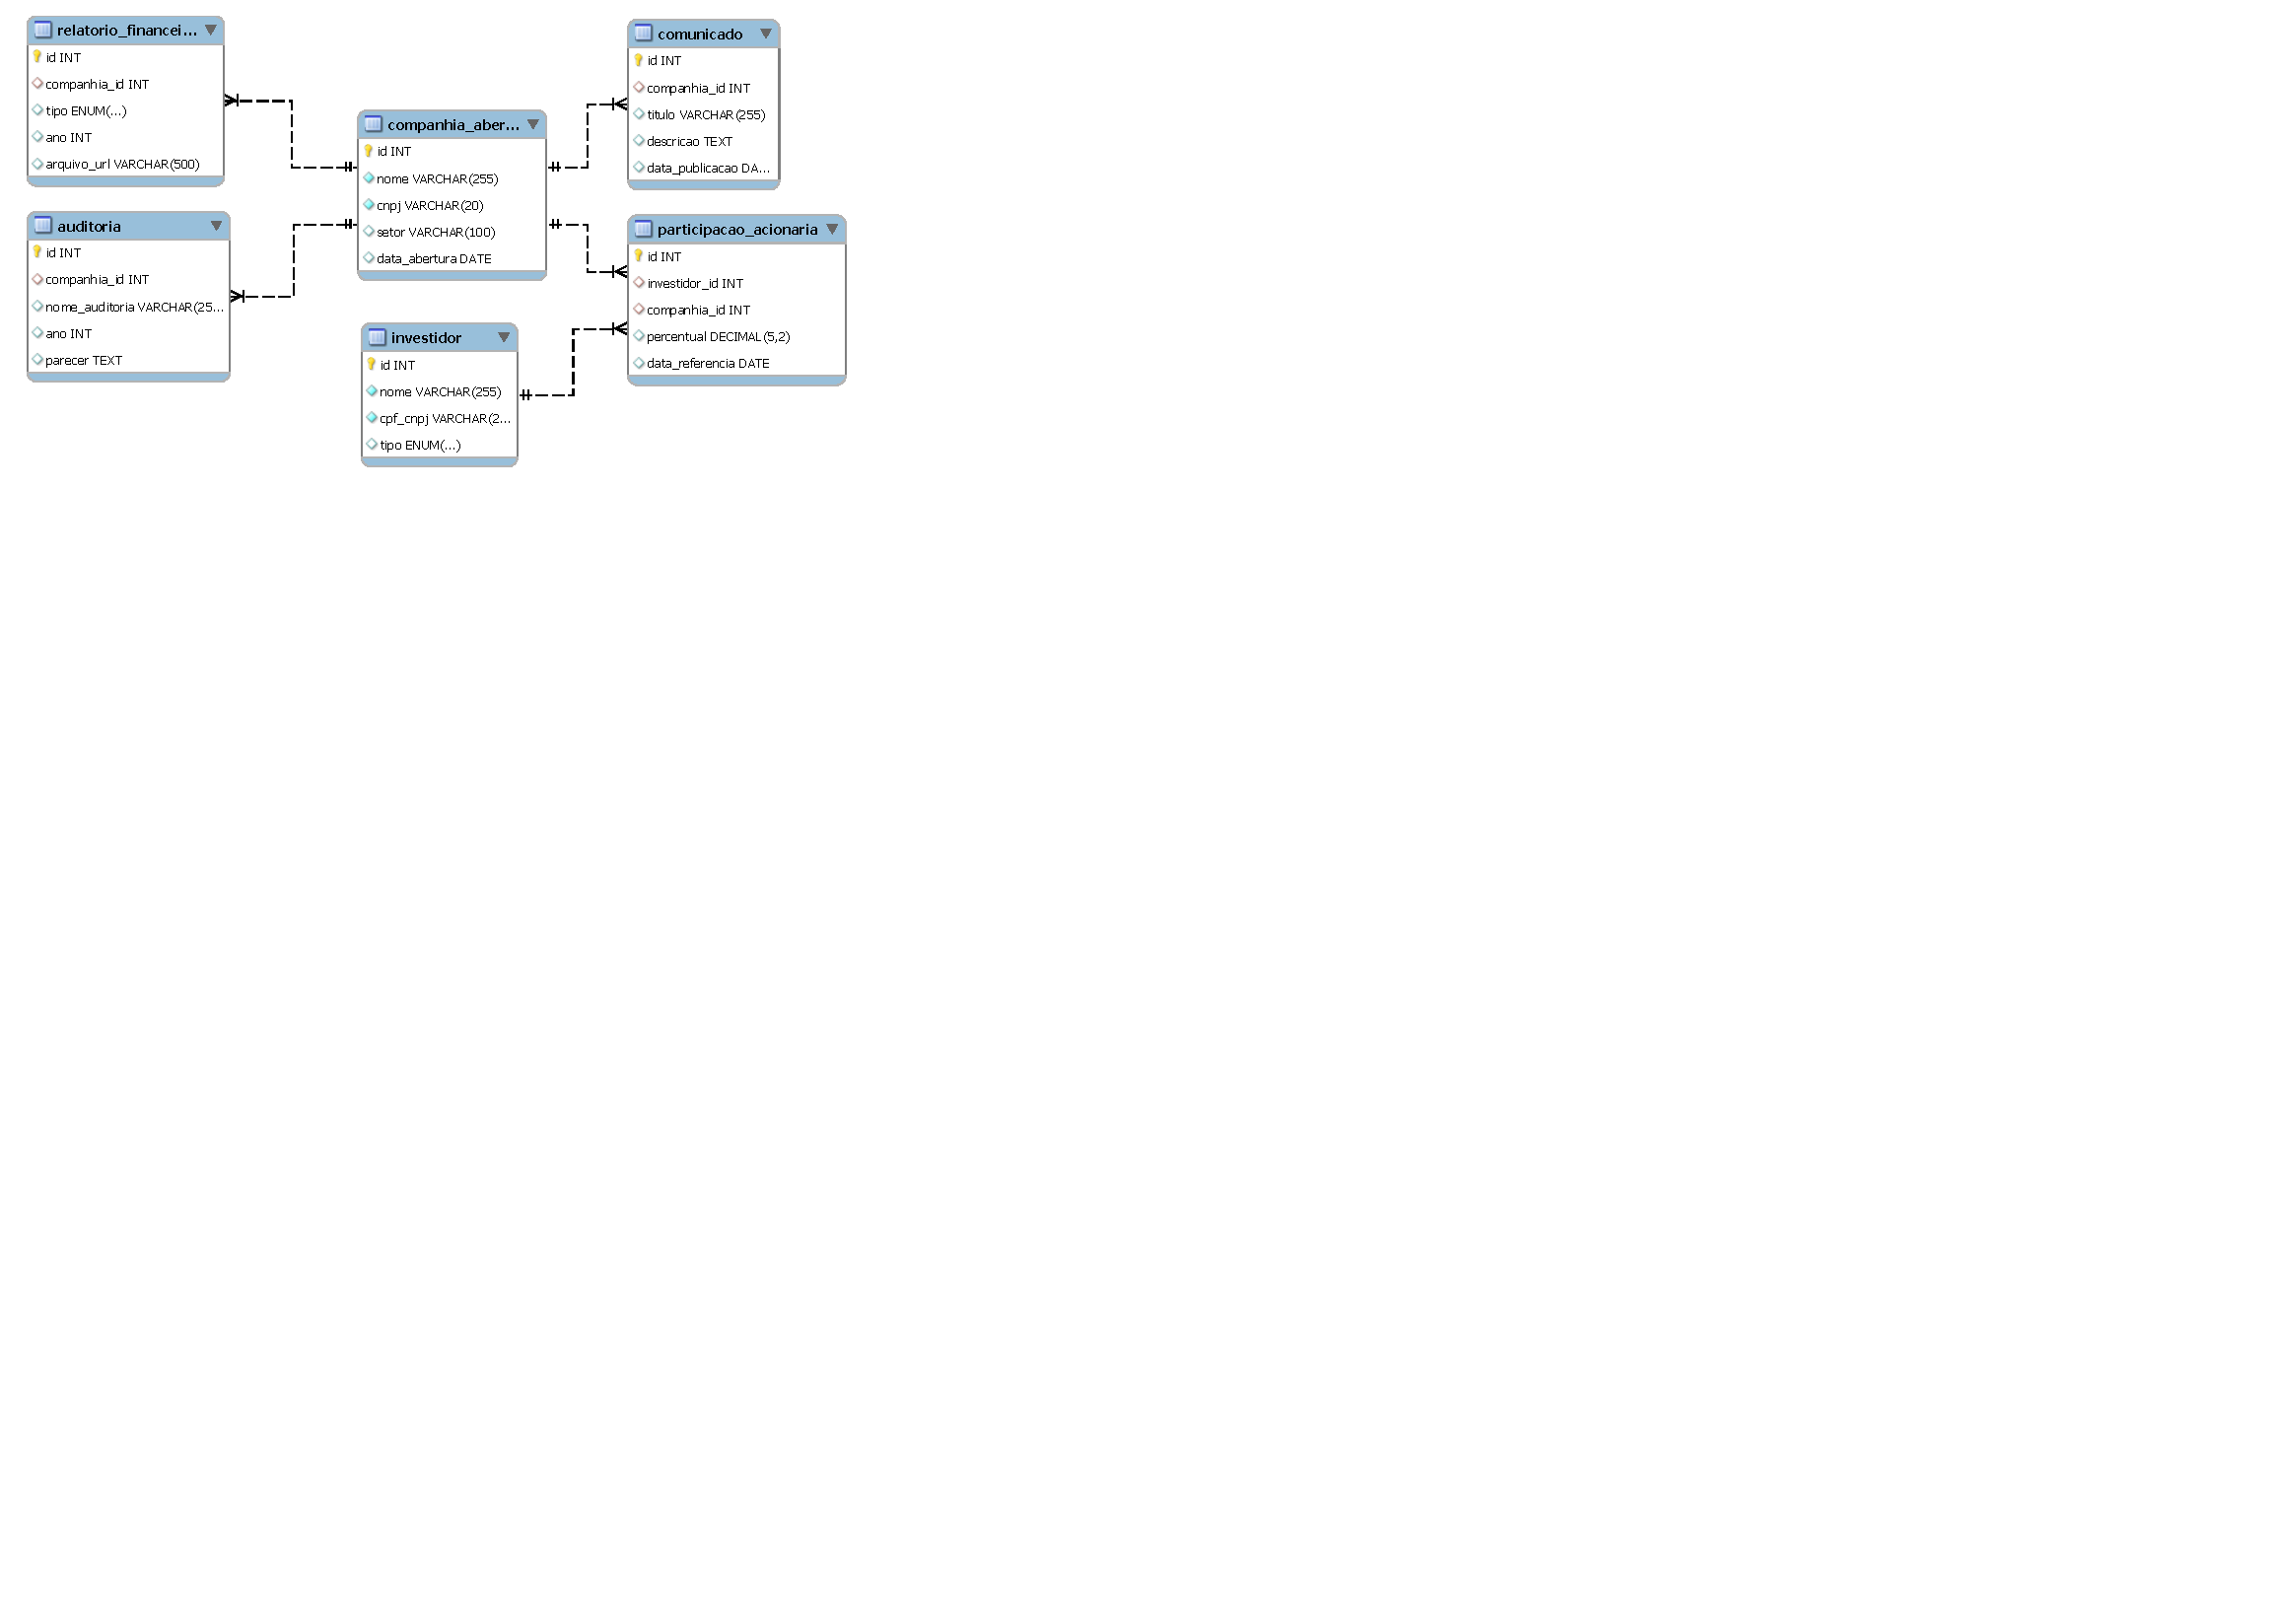
\includegraphics[width=0.9\textwidth]{figuras/esquema_logico.pdf}
	\vspace{1mm}
	\parbox[c]{0.9\textwidth}{\raggedright \legend{Elaborado pelo autor, 2024.}}
\end{figure}

O modelo proposto é composto pelas seguintes tabelas:

\begin{itemize}
	\item \textit{companhia\_aberta}
	\item \textit{comunicado}
	\item \textit{investidor}
	\item \textit{participacao\_acionaria}
	\item \textit{auditoria}
	\item \textit{relatorio\_financeiro}
\end{itemize}

A tabela \textit{companhia\_aberta} centraliza os dados cadastrais das empresas registradas na CVM, contendo atributos como \textit{nome}, \textit{cnpj}, \textit{setor} e \textit{data\_abertura}. O campo \textit{cnpj} possui uma restrição de unicidade (\textit{UNIQUE}) para garantir a integridade dos dados identificadores.

A tabela \textit{comunicado} armazena registros de publicações oficiais vinculadas às companhias, sendo referenciada pela chave estrangeira \textit{companhia\_id}, que estabelece uma relação com a tabela \textit{companhia\_aberta}. Esse vínculo viabiliza a rastreabilidade entre os comunicados e as empresas emissores.

A tabela \textit{investidor} registra os agentes que detêm participações acionárias, identificados pelo atributo \textit{cpf\_cnpj}, e categorizados segundo o tipo de investidor (\textit{Pessoa Física} ou \textit{Pessoa Jurídica}), utilizando a estrutura \textit{ENUM} para controle de domínio.

A tabela \textit{participacao\_acionaria} representa a associação entre investidores e companhias abertas, permitindo o registro da proporção de ações detidas por data de referência. Essa tabela possui chaves estrangeiras para as tabelas \textit{investidor} e \textit{companhia\_aberta}, o que possibilita a análise de composição societária ao longo do tempo.

A tabela \textit{auditoria} documenta os pareceres emitidos por empresas auditoras sobre as demonstrações financeiras das companhias, detalhando o ano do parecer, o nome da auditoria e a descrição do conteúdo emitido.

Por fim, a tabela \textit{relatorio\_financeiro} concentra os metadados dos arquivos financeiros disponibilizados pela CVM, como os Demonstrativos Financeiros Padronizados (DFP), Informações Trimestrais (ITR), o Formulário de Referência e o IAN. Cada registro inclui o tipo do documento, o ano de referência e o link para o arquivo original.

Essa estrutura relacional foi projetada visando à normalização dos dados, conforme as boas práticas de projeto de bancos de dados relacionais \cite{elmasri:2016:fundamentals}. A modelagem lógica aqui apresentada oferece a base necessária para uma integração eficiente e escalável, compatível com análises automatizadas de caráter fundamentalista. Sua implementação favorece a consistência da base de dados, o desempenho nas consultas SQL e a reutilização de componentes em diferentes módulos do sistema.



\subsection{Processo de integração de dados}

A integração de dados é um procedimento essencial que consolida informações oriundas de diversas fontes, garantindo consistência, qualidade e acessibilidade para análises estratégicas e operacionais. Esse processo transforma dados brutos em informações valiosas para a tomada de decisão e é composto por etapas interdependentes: extração, transformação e carga.

Na etapa de extração, os dados são coletados diretamente de múltiplas fontes, como os repositórios da CVM. Essa fase utiliza técnicas que asseguram a captura completa e precisa das informações, minimizando riscos de perda ou corrupção. No presente trabalho, essa etapa foi implementada por meio de \textit{scripts} automatizados em Python, que realizam o \textit{download} de arquivos compactados disponibilizados pela CVM, como o \texttt{dfp\_cia\_aberta\_2022.zip}. O sistema verifica a existência prévia dos arquivos e sua integridade antes de prosseguir com o processamento, evitando redundâncias e falhas.

Após a extração, os dados brutos passam por um processo de transformação que envolve padronização, limpeza, normalização e aplicação de regras de negócio. Essa etapa é responsável por eliminar inconsistências, corrigir valores ausentes, ajustar formatos e estruturar os dados para análises mais sofisticadas. No contexto deste projeto, foram realizadas conversões de tipos, unificação de formatos de datas e remoção de duplicidades. Informações como o código da conta contábil (\texttt{CD\_CONTA}) foram associadas às suas descrições completas com base nos planos de contas divulgados pela CVM, garantindo maior legibilidade e utilidade analítica.

Na etapa final, os dados transformados são carregados em um banco de dados relacional estruturado, visando facilitar a manipulação, a consulta e a análise posterior. Para este trabalho, optou-se pelo uso do SQLite como solução leve e eficiente, adequada ao escopo local da ferramenta desenvolvida. As tabelas foram criadas respeitando normas de integridade referencial, com chaves primárias e estrangeiras bem definidas. Dados financeiros, cadastrais e operacionais foram organizados em tabelas como \texttt{demonstrativo\_financeiro}, \texttt{informacao\_trimestral} e \texttt{empresas}, possibilitando análises temporais, cálculo de indicadores como LPA e P/L, entre outros.

A integração harmônica dessas etapas resultou em uma base de dados confiável e atualizada, que sustenta a automatização dos processos analíticos e permite a construção de modelos quantitativos e preditivos. Essa abordagem se mostra fundamental para a aplicação da análise fundamentalista no contexto do mercado financeiro, proporcionando uma visão estruturada e estratégica para a tomada de decisão \cite{costa:2024:integraccao, halevy:2006:data}.

\section{Estado da arte} \label{sec:estado-arte}

Nesta seção, são analisados os principais estudos acadêmicos e projetos práticos que fundamentam a abordagem deste trabalho. Inicialmente, apresenta-se uma síntese dos trabalhos existentes, destacando seus objetivos, metodologias empregadas e limitações encontradas. Em seguida, evidencia-se como o presente estudo propõe uma integração inédita de dados e técnicas, superando as deficiências das abordagens anteriores.

\subsection{Trabalhos acadêmicos}

Os estudos acadêmicos voltados à modelagem e à análise de dados financeiros têm se concentrado na automatização da análise fundamentalista e na adaptação de modelos tradicionais ao contexto do mercado brasileiro. Por exemplo, \citet{montoia:2021:automatizaccao} desenvolvem um sistema automatizado para a análise de ações, enfatizando a melhoria na rapidez e na eficiência da tomada de decisões. Esse trabalho detalha a aplicação de algoritmos de processamento de dados que reduzem a intervenção manual, permitindo uma análise em tempo real dos indicadores financeiros.

De forma complementar, \citet{deAraujo:2021:modelo} propôs um modelo flexível que adapta os conceitos da análise fundamentalista para refletir as particularidades dos dados nacionais, considerando variáveis específicas do mercado brasileiro. Esse estudo destaca a importância da customização dos parâmetros e a integração de variáveis macroeconômicas na modelagem financeira.

Além disso, \citet{delalibera:2023:automatizaccao} aprimorou metodologias tradicionais, como o Modelo Rojo, para avaliação de ativos, enfatizando a precisão na quantificação de riscos e oportunidades de investimento. Este trabalho apresenta uma abordagem robusta que combina técnicas estatísticas com algoritmos de \textit{machine learning} para melhorar a acurácia das previsões. Por sua vez, \citet{reis:2020:analise} investigou a aplicação prática desses métodos na análise das ações negociadas, proporcionando \textit{insights} sobre a volatilidade do mercado e a relevância de diferentes indicadores financeiros.

Outros estudos, como o de \citet{vieira:2019:montagem}, analisam estratégias de montagem de carteiras de ações, comparando a performance das carteiras com índices de mercado e ressaltando as dificuldades na diversificação e no balanceamento dos ativos. Da mesma forma, \citet{freitas:2020:analise} explorou a aplicação criteriosa de indicadores no setor bancário, evidenciando os desafios em medir a solidez financeira e a eficiência operacional de instituições financeiras.

\subsection{Projetos e plataformas similares}

No campo dos projetos práticos, diversas iniciativas presentes em repositórios, especialmente no GitHub, vêm se destacando por oferecer ferramentas e bases de dados voltadas para a extração e análise de informações financeiras. Por exemplo, o projeto de \citet{paiva:2025:projetoGitHub} apresenta um sistema integrado que coleta, processa e organiza dados contábeis de empresas. Essa ferramenta tem como objetivo facilitar a aplicação da análise fundamentalista ao disponibilizar dados de forma estruturada e acessível, promovendo maior transparência e facilidade na análise dos balanços.

De maneira similar, \citet{minas:2025:projetoGitHub} propõe uma abordagem inovadora para a análise de balanços empresariais, enfatizando a importância da normalização dos dados e da criação de indicadores personalizados que se ajustem às especificidades de cada setor. Repositórios como os de \citet{fontinele:2025:projetoGitHub} e \citet{louredo:2025:projetoGitHub} se destacam ao desenvolver ferramentas específicas para interpretar demonstrações financeiras a partir de dados públicos, permitindo que o usuário identifique rapidamente pontos críticos e oportunidades de investimento. Contudo, grande parte dessas iniciativas se restringe à coleta e ao processamento dos dados, sem oferecer uma análise histórica contínua que possibilite a compreensão das tendências de longo prazo.

\subsection{Diferencial do trabalho proposto}

O diferencial do presente trabalho reside na integração de um histórico abrangente de dados financeiros com um sistema automatizado de acesso e análise das informações públicas disponibilizadas pela CVM. Embora os experimentos realizados tenham utilizado um recorte temporal de cinco anos, a ferramenta não se limita a esse intervalo. Enquanto a CVM mantiver a estrutura dos dados em seus repositórios, o sistema permanecerá funcional e poderá ser continuamente alimentado com novos dados, garantindo sua atualização e longevidade.

A proposta se distingue, ainda, por tratar-se de uma solução de código aberto, o que permite sua auditoria, personalização e extensão por outros pesquisadores e profissionais interessados. Essa abertura favorece a colaboração contínua, possibilitando o aprimoramento da ferramenta e sua adaptação a novos contextos analíticos ou setores econômicos específicos.

A abordagem adotada neste trabalho viabiliza tanto a avaliação contínua e comparativa dos dados quanto a análise contextualizada das informações. A avaliação contínua é sustentada pelo acúmulo de dados históricos, o que permite identificar tendências e padrões relevantes ao longo do tempo. Já a análise contextualizada emerge da capacidade de combinar dados históricos e atuais, ampliando a compreensão sobre ciclos econômicos, sazonalidades e eventos que impactam o mercado.

As principais inovações e contribuições do sistema desenvolvido podem ser resumidas nos seguintes pontos:

\begin{itemize}
	\item integração de dados históricos financeiros em larga escala;
	\item processamento automatizado, com foco em escalabilidade e reusabilidade;
	\item contextualização dos indicadores contábeis e financeiros;
	\item manutenção da funcionalidade do sistema diante de novas atualizações da CVM, desde que preservada a estrutura de dados;
	\item disponibilização em formato de código aberto, fomentando a transparência e a colaboração.
\end{itemize}

Ao superar as limitações de iniciativas anteriores, que se restringem majoritariamente à coleta e estruturação pontual dos dados, a solução apresentada promove uma abordagem sistemática e extensível, capaz de subsidiar análises fundamentalistas robustas e atualizadas. Essa característica torna o sistema especialmente útil para aplicações acadêmicas, institucionais e profissionais voltadas à tomada de decisão baseada em fundamentos econômicos e financeiros.

\chapter{METODOLOGIA}
Esta seção apresenta a metodologia de execução do presente trabalho.
A Seção \ref{subsec:classificacao} define o escopo e os objetivos deste trabalho, delineando as principais áreas de investigação.
Em seguida, a Seção \ref{subsec:metodologia} descreve as abordagens e técnicas utilizadas para planejar e conduzir o desenvolvimento da ferramenta proposta.
Por fim, a Seção \ref{subsec:solucao} detalha os passos do trabalho, incluindo a investigação da estrutura dos dados, a modelagem lógica e o desenvolvimento da ferramenta de integração de dados.

\section{Classificação da Pesquisa} \label{subsec:classificacao}

Para fundamentar a classificação metodológica da pesquisa, foram consultadas as obras de \citet{cervo:1983:metodologia}, que apresentam diferentes abordagens científicas, e de \citet{gerhardt:2009:metodos}, que tratam de métodos amplamente utilizados na pesquisa acadêmica.

Quanto à natureza, esta pesquisa é aplicada, pois busca resolver um problema prático relacionado à integração automatizada de dados financeiros públicos disponibilizados pela CVM, promovendo avanços na análise fundamentalista e no apoio à tomada de decisão.

Em relação aos objetivos, a investigação é exploratória e descritiva. A parte exploratória está ligada à compreensão da estrutura dos dados da CVM, enquanto o aspecto descritivo se manifesta na proposição e implementação de uma ferramenta que permita o uso prático dessas informações de forma organizada.

Os procedimentos técnicos combinam pesquisa bibliográfica e documental para levantamento e compreensão teórica dos dados públicos, juntamente com o desenvolvimento de uma solução tecnológica que automatiza sua coleta, integração e disponibilização.

A abordagem metodológica adotada é mista. Aspectos qualitativos estão presentes na análise estrutural e na modelagem dos dados, enquanto os elementos quantitativos se refletem no processamento automatizado e na organização das informações em larga escala.

No contexto da área de Computação, a pesquisa representa o desenvolvimento de uma solução tecnológica voltada à resolução de um problema específico, com potencial de aplicação prática no meio acadêmico e no ambiente de análise financeira \cite{wazlawick:2009:metodo}.


\section{Gerenciamento do Projeto} \label{subsec:metodologia}

O gerenciamento deste projeto foi conduzido com base em práticas ágeis de desenvolvimento de software, adotando a metodologia \textit{Scrum} como estrutura principal \cite{schwaber:2004:agile}. Como apoio visual, utilizou-se também o quadro de sinalização \textit{Kanban}, contribuindo para a organização e o acompanhamento do fluxo de trabalho \cite{anderson:2010:kanban}.

Ambas as abordagens foram aplicadas de forma adaptada às necessidades do projeto, considerando sua natureza acadêmica e o escopo restrito da equipe envolvida. O \textit{Scrum} foi utilizado de maneira personalizada, com ciclos iterativos de duas semanas, denominados \textit{sprints}, nos quais as tarefas foram definidas, priorizadas e acompanhadas ao longo do desenvolvimento \cite{sutherland:2014:scrum}.

O Kanban complementou esse processo, funcionando como ferramenta visual para monitoramento das atividades, identificação de gargalos e ajustes de fluxo, contribuindo para uma gestão mais eficiente \cite{hammarberg:2014:kanban}. Essa combinação flexível e adaptada de métodos ágeis mostrou-se eficaz para garantir a organização, a visibilidade do progresso e a entrega incremental da solução proposta.



\section{Solução proposta}  \label{subsec:solucao}

O ponto de partida do projeto consistiu em uma investigação detalhada da estrutura dos dados disponibilizados pela CVM. Essa etapa contemplou a análise dos formatos de arquivos, dos tipos de dados disponíveis e dos métodos de acesso às informações públicas fornecidas por essa instituição.

Embora os dados da B3 não tenham sido utilizados diretamente na construção da ferramenta, sua presença no contexto do mercado de capitais justificou a compreensão de sua estrutura e funcionamento. Dessa forma, foram consultados documentos como o relatório anual da CVM \cite{cvm:2023:relatorioanual} e referências sobre a estrutura de dados da B3 \cite{b3:2023:estruturadados}, a fim de mapear desafios e possibilidades associados à integração de dados financeiros.

A Figura \ref{fig:fluxograma} ilustra o fluxo geral do projeto. A fase inicial compreendeu a coleta e documentação dos dados da CVM, seguida pela modelagem lógica que estruturou um banco de dados unificado, preparado para integração e análise posterior.

\begin{figure}[!htb] \centering
	\caption{Fluxograma do projeto} \label{fig:fluxograma}
	\begin{varwidth}{\linewidth}
		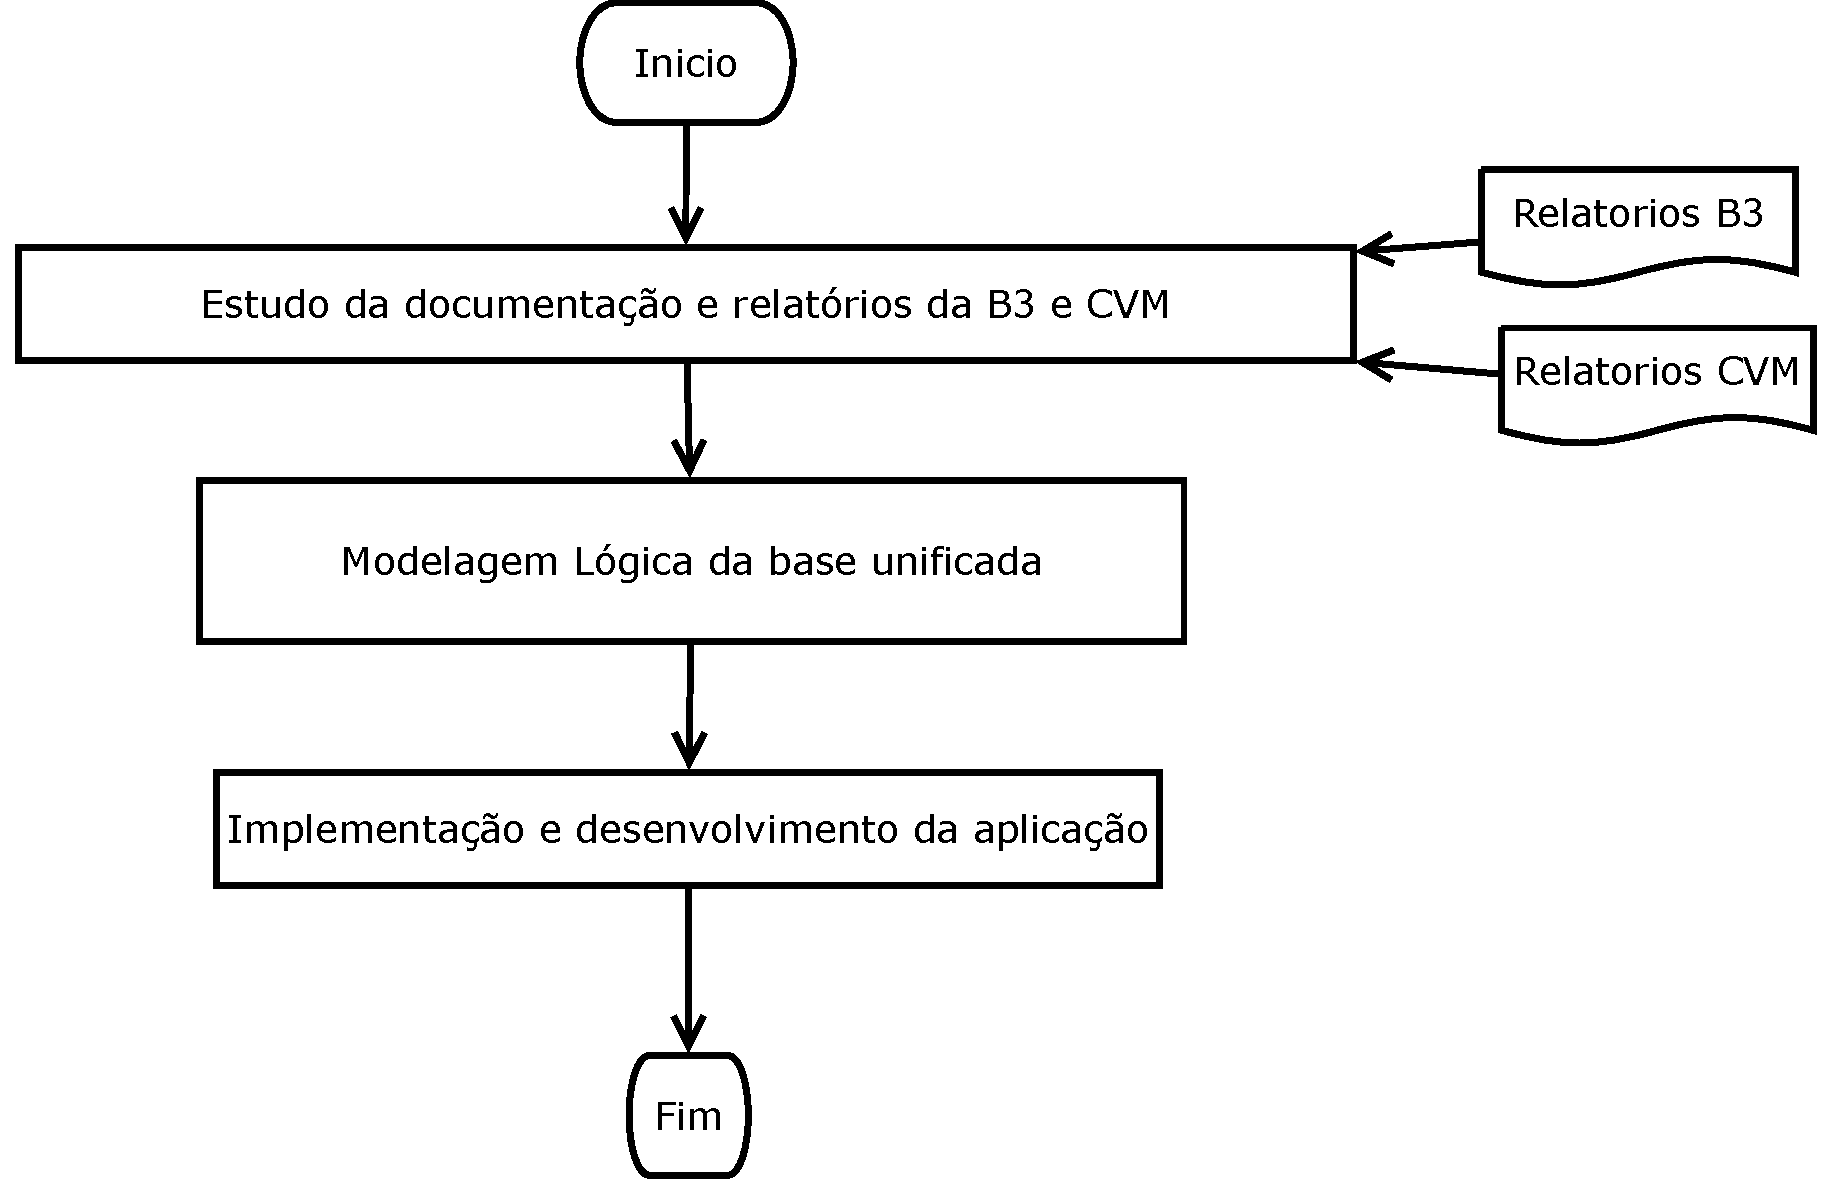
\includegraphics[width=0.6\textwidth]{figuras/fluxograma - v3.pdf}
		\legend{Elaborado pelo autor, 2024.}
	\end{varwidth}
\end{figure}

Com base na análise inicial, foi realizada a modelagem lógica da base de dados, com foco na criação de um esquema unificado que contemplasse as diferentes estruturas contábeis e financeiras presentes nos arquivos da CVM. Para essa etapa, foram consideradas boas práticas descritas na literatura sobre modelagem de dados financeiros \cite{domingues:2020:modelagem} e integração de grandes volumes de dados \cite{perlin:2021:analise}.

A etapa seguinte consistiu no desenvolvimento da aplicação de software responsável por automatizar o processo de coleta, tratamento e inserção dos dados na base unificada. Essa ferramenta foi desenvolvida com tecnologias modernas de extração e processamento de dados, garantindo flexibilidade e desempenho.

A aplicação foi capaz de realizar o \textit{download} dos arquivos disponibilizados pela CVM, aplicar os tratamentos necessários para padronização e limpeza dos dados, e armazená-los de forma estruturada. Esse processo assegurou a integridade das informações e facilitou seu uso em análises fundamentalistas, estudos acadêmicos e outras aplicações. A proposta esteve alinhada com práticas consolidadas no desenvolvimento de soluções para automação e análise de dados \cite{prikladnicki:2014:desenvolvimentosoftware} \cite{nhimi:2016:desenvolvimentosoftware}.


\section{Materiais e Tecnologias} \label{subsec:material}

Esta seção apresenta os materiais e tecnologias que serão empregados durante o desenvolvimento do trabalho.  
O projeto será desenvolvido em um computador desktop cujas especificações são apresentadas no Quadro \ref{tab:specs-tcc}.  


\begin{board}[!htb]  \centering
	\caption{Especificações do computador utilizado no TCC}
	\label{tab:specs-tcc}
	\begin{varwidth}{\linewidth}
		\begin{tabular}{|p{4cm}|p{11cm}|} \hline
			\textbf{Componente} & \textbf{Especificação} \\ \hline
			Processador & AMD Ryzen 5 5600G, 6-Core, 12-Threads, 3.6GHz (4.6GHz Turbo), Cache 19MB, AM4 \\ \hline  
			Memória RAM & 2x Kingston Fury Beast, 16GB, 3200MHz, DDR4, CL16 \\ \hline  
			Armazenamento & SSD TGT Seal ST, 240GB, Sata III, Leitura 500 MB/s, Gravação 450 MB/s \\  
			& HD WD Blue, 1TB, 3.5, 5400 RPM, Sata III, Cache 64MB \\ \hline  
			Sistema Operacional & Windows 11 Pro \\ \hline
		\end{tabular}
		\legend{Elaborado pelo autor, 2024.}
	\end{varwidth}
\end{board}

Durante a modelagem do banco de dados, utilizou-se o MySQL Workbench\footnote{\url{https://www.mysql.com/products/workbench/}}, versão 8.0. Essa ferramenta permitiu a criação visual do esquema lógico, facilitando o planejamento e a organização das entidades e relacionamentos.

Contudo, para o desenvolvimento da aplicação, optou-se pelo uso do SQLite\footnote{\url{https://www.sqlite.org/}}, versão 3.49.1, como solução de banco de dados local. O SQLite foi adotado como banco de dados padrão do sistema, por oferecer maior praticidade na integração com o código desenvolvido. Sua leveza, portabilidade e independência de um servidor o tornam especialmente adequado para o uso do código por estudantes e profissionais da área financeira.

A linguagem de programação utilizada foi o Python, na versão 3.12.9\footnote{\url{https://www.python.org/downloads/release/python-3129/}}, pela sua versatilidade, ampla comunidade e bibliotecas especializadas.

As bibliotecas utilizadas no projeto foram:

\begin{itemize}
	\item Pandas, versão 2.2.1\footnote{\url{https://pandas.pydata.org/}}
	\item Numpy, versão 1.26.4\footnote{\url{https://numpy.org/}}
	\item Beautifulsoup4, versão 4.12.2\footnote{\url{https://www.crummy.com/software/BeautifulSoup/}}
	\item Lxml, versão 5.1.0\footnote{\url{https://lxml.de/}}
	\item Requests, versão 2.31.0\footnote{\url{https://requests.readthedocs.io/en/latest/}}
	\item SQLAlchemy, versão 2.0.27\footnote{\url{https://www.sqlalchemy.org/}}
	\item Mysql-Connector-Python, versão 8.3.0\footnote{\url{https://dev.mysql.com/downloads/connector/python/}}
\end{itemize}

A biblioteca \textit{pandas} foi empregada para manipulação e análise de dados tabulares. Sua estrutura baseada em \textit{DataFrames} proporcionou uma forma eficiente de organizar, filtrar e agrupar informações financeiras.

A biblioteca \textit{numpy} foi utilizada em conjunto com o pandas para operações numéricas vetoriais e matriciais, fundamentais na realização de cálculos e no tratamento de grandes volumes de dados.

Para extração de informações de páginas web, foi utilizada a biblioteca \textit{beautifulsoup4}, que permitiu navegar pela estrutura HTML de documentos e extrair dados de forma precisa. A ela foi integrada a biblioteca \textit{lxml}, que serviu como parser rápido e eficiente de HTML e XML.

A coleta dos dados disponibilizados pela CVM foi realizada por meio da biblioteca \textit{requests}, que viabilizou a comunicação com serviços HTTP e o \textit{download} automatizado das informações necessárias.

A interface com o banco de dados foi desenvolvida com o auxílio do \textit{SQLAlchemy}, que forneceu abstração e controle sobre as operações de inserção, consulta e atualização dos dados no SQLite, utilizando o paradigma de mapeamento objeto-relacional.

Durante os testes iniciais com a estrutura modelada no MySQL, foi utilizada a biblioteca \textit{mysql-connector-python}, o conector oficial do MySQL para Python. Essa ferramenta garantiu a compatibilidade entre a modelagem relacional inicial e os scripts desenvolvidos, possibilitando a validação funcional da estrutura antes da migração definitiva para o SQLite.
%TODO - a mexer
\chapter{DESENVOLVIMENTO}

Este capítulo apresenta o processo de desenvolvimento da ferramenta proposta para a coleta, estruturação e integração de dados financeiros públicos disponibilizados pela CVM, com foco em análises fundamentalistas de companhias abertas brasileiras. A escolha pelo banco de dados SQLite justifica-se por sua leveza, portabilidade e facilidade de integração com sistemas locais, características adequadas a estudos exploratórios e reprodutíveis.

As atividades foram organizadas em três frentes principais, que estruturam as seções deste capítulo. A Seção~\ref{sec:analise_cvm} descreve a análise preliminar dos dados disponibilizados pela CVM, com destaque para a identificação de padrões, inconsistências e limitações nos metadados. A Seção~\ref{sec:modelagem} detalha a modelagem e estruturação da base de dados, com ênfase na padronização relacional e na aplicação de boas práticas de modelagem para contextos financeiros, conforme discutido na literatura \cite{elmasri:2016:fundamentals}. Por fim, a Seção~\ref{sec:software} apresenta o sistema desenvolvido em Python, incluindo os módulos responsáveis pela coleta, transformação e armazenamento dos dados, bem como os mecanismos de registro de eventos (\textit{logs}).


\section{Análise inicial dos dados da CVM} \label{sec:analise_cvm}

A primeira etapa consistiu na compreensão do formato, da frequência de atualização e de outros aspectos relevantes relacionados aos dados disponibilizados pela CVM. Como o foco do trabalho são as Companhias (CIA) Abertas\footnote{\url{https://dados.cvm.gov.br}}, realizou-se uma análise do site como fonte para obtenção dessas informações. A partir disso, foram identificados os conjuntos de dados referentes às Companhias Abertas, organizados nas seguintes pastas:

\begin{itemize}
	\item informação cadastral;
	\item formulário cadastral (FCA);
	\item periódicos e eventuais (IPE);
	\item formulário de referência (FRE);
	\item valores mobiliários negociados e detidos (VLMO);
	\item formulário de informações trimestrais (ITR);
	\item formulário de demonstrações financeiras padronizadas (DFP);
	\item informe do código de governança (ICBGC).
\end{itemize}

As informações cadastrais compõem uma categoria distinta, classificada como cadastro (CAD), enquanto os demais arquivos são agrupados sob a categoria de documentos (DOC). Ao acessar o site de dados da CVM\footnote{\url{https://dados.cvm.gov.br/dados/}}, especificamente a seção referente às Companhias Abertas, é possível visualizar essas duas categorias de dados.

Será apresentada, a seguir, a descrição de cada pasta referente ao conjunto de dados da CVM da CIA Aberta, com a finalidade de esclarecer o conteúdo e a utilidade de cada uma.

\subsection{Informação cadastral} 
O conjunto Informação Cadastral reúne os dados cadastrais das companhias abertas disponibilizados pela CVM. Entre as informações disponibilizadas, destacam-se o número do Cadastro Nacional da Pessoa Jurídica (CNPJ), a data de registro da companhia e a situação atual desse registro. Esses dados são fundamentais para análises regulatórias, econômicas e financeiras, além de servirem como base para estudos acadêmicos e pesquisas de mercado. O dicionário de dados, disponibilizado em formato textual, contém a descrição detalhada das colunas e dos tipos de dados presentes no arquivo principal. Já os dados propriamente ditos, que contêm os registros cadastrais das companhias abertas, são apresentados em um arquivo estruturado.

Este conjunto de dados é de acesso público e está disponível na plataforma de dados abertos da CVM. A base foi originalmente criada em 17 de setembro de 2017, e desde então é atualizada diariamente. Integra a base de dados denominada Cadastro de Regulados, o que reforça seu caráter institucional e sua relevância para fins de controle e transparência regulatória.

\subsection{Formulário cadastral (FCA)}
O FCA é um documento eletrônico cuja entrega periódica ou eventual é regulamentada pelo a \citet{cvm:2022:resolucao}. Este formulário deve ser enviado à CVM por meio do sistema \textit{Empresas.NET}, sendo uma obrigação regulatória destinada às companhias abertas. Sua principal função é atualizar e manter organizadas as informações institucionais e operacionais dessas entidades. O conjunto de dados públicos relacionados ao Formulário de Referência Anual (FCA), disponibilizado pela CVM, apresenta-se organizado em duas categorias principais de informações: os endereços de \textit{download} dos documentos completos submetidos pelas companhias abertas e os conteúdos estruturados das seções que compõem o formulário.

A primeira categoria refere-se ao arquivo \texttt{fca\_cia\_aberta}, que contém os links para o \textit{download} dos documentos completos entregues pelas companhias nos últimos cinco anos. A visualização desses documentos requer a utilização do programa \textit{Empresas.NET}, disponibilizado pela própria CVM. A segunda categoria compreende os conteúdos integrais do formulário, apresentados em formato estruturado e organizados em arquivos distintos que refletem as diversas seções. Entre os arquivos disponibilizados, destacam-se: 
\begin{itemize}
	\item \texttt{fca\_cia\_aberta\_geral};
	\item \texttt{fca\_cia\_aberta\_pais\_estrangeiro\_negociacao};
	\item \texttt{fca\_cia\_aberta\_canal\_divulgacao};
	\item \texttt{fca\_cia\_aberta\_endereco};
	\item \texttt{fca\_cia\_aberta\_valor\_mobiliario};
	\item \texttt{fca\_cia\_aberta\_auditor};
	\item \texttt{fca\_cia\_aberta\_escriturador};
	\item \texttt{fca\_cia\_aberta\_dri};
	\item \texttt{fca\_cia\_aberta\_departamento\_acionistas}. 
\end{itemize}

Cada um desses arquivos aborda uma seção específica do formulário, possibilitando a segmentação e a análise detalhada das informações declaradas pelas companhias abertas. Os arquivos são atualizados semanalmente, refletindo tanto novas entregas quanto reapresentações realizadas pelas companhias reguladas. Além disso, mantém-se um histórico contínuo desde o ano de 2010, incluindo inclusive arquivos que não estão sujeitos à política de atualização vigente. O dicionário de dados correspondente é disponibilizado em formato compactado e oferece descrições detalhadas de todas as colunas e variáveis presentes nos arquivos.

Para fins de análise temporal e organização, os formulários referentes aos anos de 2020 a 2025 encontram-se agrupados em arquivos anuais distintos. Este conjunto de dados integra a base denominada \textit{Documentos Periódicos e Eventuais de Regulados}, cuja criação remonta a 29 de maio de 2020. Sua manutenção ocorre de forma semanal, assegurando a atualização constante das informações disponibilizadas.

\subsection{Periódicos e Eventuais (IPE)}

O conjunto de dados referente às Informações Periódicas e Eventuais (IPE) reúne documentos não estruturados enviados por companhias abertas à Comissão de Valores Mobiliários (CVM), abrangendo os últimos cinco anos. Esses documentos, de caráter regulatório, contemplam tanto as obrigações periódicas quanto as comunicações eventuais exigidas ao longo das atividades societárias e da interlocução com o mercado. Trata-se de um acervo robusto, que reflete a diversidade de exigências legais e normativas aplicáveis às companhias reguladas. O conteúdo do conjunto está organizado em seis grandes categorias documentais:

\begin{itemize}
	\item governança e estrutura societária;
	\item relação com investidores e mercado;
	\item informações econômico-financeiras e contábeis;
	\item transações e operações societárias;
	\item companhias em situação especial;
	\item informações regulatórias específicas.
\end{itemize}

A categoria de governança e estrutura societária compreende documentos que regulam a organização interna e as diretrizes de conduta das companhias, como Acordos de Acionistas, Estatutos Sociais, Regimentos Internos, Códigos de Conduta, além de Políticas de Governança e Sustentabilidade. Esses registros são fundamentais para garantir a conformidade, a transparência e a integridade das práticas de gestão corporativa. Já os documentos de relação com investidores e mercado incluem comunicados oficiais direcionados ao público investidor e à sociedade, como Comunicados ao Mercado, Avisos a Acionistas e Debenturistas, Fatos Relevantes, Informações prestadas a bolsas estrangeiras e o Calendário de Eventos Corporativos. Tais documentos asseguram a divulgação tempestiva e adequada de informações relevantes, conforme exigido pelas normas da CVM.

No que se refere às informações econômico-financeiras e contábeis, o conjunto abrange dados sobre a situação patrimonial e os resultados das companhias, além de instrumentos financeiros e políticas de distribuição de lucros. Incluem-se nessa categoria Demonstrativos Financeiros, Documentos de Ofertas Públicas, Escrituras de Debêntures, Políticas de Dividendos e de Destinação de Resultados. A categoria de transações e operações societárias, por sua vez, contém registros de eventos relevantes que impactam a estrutura e o capital das empresas, como Comunicações sobre Transações com Partes Relacionadas, Ofertas Públicas de Aquisição (OPA) e Planos de Remuneração Baseados em Ações. Já a documentação relativa a companhias em situação especial reúne informações sobre empresas que enfrentam processos de falência, liquidação ou recuperação judicial/extrajudicial, sendo essenciais para análise de risco e monitoramento da situação jurídico-financeira dessas entidades. Por fim, a categoria de informações regulatórias específicas abrange documentos exigidos por normativos da CVM, como as comunicações sobre negociação de valores mobiliários por pessoas ligadas, políticas de atuação de auditores independentes e outras políticas internas obrigatórias.

Os documentos estão organizados por ano de entrega, reunindo todas as submissões realizadas em cada período. Os arquivos correspondentes ao ano corrente e ao ano imediatamente anterior (A-1) são atualizados semanalmente, incorporando novas submissões e reapresentações. O conjunto conta com um histórico completo desde 2003, incluindo arquivos legados que, embora não estejam sujeitos à política atual de atualização contínua, permanecem acessíveis. As edições anuais estão disponíveis de 2020 a 2025, cada uma distribuída em arquivos compactados contendo os documentos entregues pelas companhias abertas no respectivo ano. A descrição das colunas e variáveis utilizadas na indexação e organização dos dados está disponível em um dicionário de dados no formato textual. O conjunto foi instituído em 27 de fevereiro de 2021 e segue uma política de atualização semanal, com base nos \textit{Documentos Periódicos e Eventuais de Regulados} recebidos pela CVM.

\subsection{Formulário de Referência (FRE)}

O Formulário de Referência (FRE) é um documento eletrônico previsto na \citet{cvm:2022:resolucao}, cuja apresentação à Comissão de Valores Mobiliários (CVM) é obrigatória e periódica (ou, em alguns casos, eventual), sendo realizada por meio do sistema \textit{Empresas.NET}. A principal finalidade do FRE é consolidar e divulgar, de forma padronizada, um conjunto abrangente de informações sobre o emissor, abrangendo sua estrutura societária, situação financeira, práticas de governança, riscos e relação com o mercado.

O conjunto de dados público associado ao FRE disponibiliza tanto os endereços para \textit{download} dos formulários quanto o conteúdo estruturado desses documentos em formato tabular. As duas principais componentes desse conjunto são:

\begin{itemize}
	\item endereços para \textit{download} dos formulários;
	\item conteúdo estruturado dos formulários em formato CSV.
\end{itemize}

O primeiro item refere-se aos links para \textit{download} dos formulários entregues pelas companhias abertas nos últimos cinco anos, disponíveis por meio do conjunto \texttt{fre\_cia\_aberta}. A visualização dos arquivos requer o uso do programa Empresas.NET, distribuído gratuitamente pela CVM. Já o segundo item diz respeito ao conteúdo dos formulários em formato estruturado, disponibilizado em arquivos estruturados. Esses arquivos abrangem diversas dimensões informacionais, organizadas nos seguintes grupos:

\begin{itemize}
	\item informações institucionais e operacionais;
	\item aspectos financeiros e patrimoniais;
	\item administração e governança;
	\item ações e mercado;
	\item aspectos sociais e de diversidade.
\end{itemize}

As informações institucionais e operacionais reúnem dados centrais sobre a estrutura e composição da companhia. Entre os principais elementos estão a identificação dos administradores, os dados do auditor independente, a estrutura de participação societária, os ativos imobilizados e intangíveis e o enquadramento da empresa em grupos econômicos. Esses dados permitem compreender a organização corporativa da companhia, sua capacidade operacional e seu posicionamento no mercado.

No que se refere aos aspectos financeiros e patrimoniais, o conteúdo cobre o endividamento da empresa, a política de distribuição de dividendos, a composição e evolução do capital social, bem como os direitos associados às ações emitidas. Também são informadas as obrigações assumidas, as operações com valores mobiliários e as movimentações relevantes no patrimônio da empresa. Essas informações são fundamentais para a análise da saúde financeira da companhia e sua relação com investidores, credores e o mercado de capitais.

A seção de administração e governança fornece uma visão detalhada da estrutura decisória da companhia, incluindo a composição dos conselhos e comitês, os vínculos entre administradores, as políticas de remuneração — fixas e variáveis — e as práticas de governança corporativa. Também são disponibilizadas informações sobre as políticas internas que regulam a negociação de valores mobiliários por parte dos administradores, o que contribui para a avaliação do grau de transparência e adesão da empresa a boas práticas de mercado. Já a seção de ações e mercado trata da estrutura acionária da companhia, descrevendo a distribuição do capital social, a existência de programas de ADRs e a negociação de ações em bolsas internacionais, permitindo avaliar o grau de internacionalização da empresa.

Introduzidos a partir da versão de 2023 do formulário, os aspectos sociais e de diversidade ampliam o escopo informacional ao incluir dados sobre o perfil dos empregados e da administração com base em critérios como gênero, raça, faixa etária e localização geográfica. A incorporação desses elementos reflete a crescente importância da agenda ESG (ambiental, social e de governança) e reforça o papel da diversidade e da responsabilidade social na estratégia e reputação institucional das companhias abertas.

Os arquivos do FRE são atualizados semanalmente, incluindo tanto novas submissões quanto reapresentações realizadas pelas companhias. O conjunto mantém um histórico contínuo a partir de 2010. Os arquivos estruturados são acompanhados por um dicionário de dados, fornecido em formato compactado, que descreve detalhadamente as variáveis e colunas presentes nos arquivos. Além disso, estão disponíveis edições anuais consolidadas do conjunto, organizadas em pacotes compactados que abrangem os anos de 2020 a 2025, facilitando análises históricas e comparativas. O conjunto foi criado em 3 de novembro de 2019 e sua atualização é feita com frequência semanal, a partir da base de \textit{Documentos Periódicos e Eventuais de Regulados} submetidos à CVM.


\subsection{Valores mobiliários negociados e detidos (VLMO)}
O conjunto de dados VLMO contempla informações de envio obrigatório à CVM, conforme a Resolução \citet{cvm:2021:resolucao44}. Trata-se de uma obrigação de natureza periódica, cujo cumprimento deve ser realizado pelas companhias abertas por meio do sistema eletrônico \textit{Empresas.NET}. Esse conjunto tem como objetivo registrar e divulgar, de maneira transparente, a posição e as negociações realizadas com valores mobiliários por administradores, membros do conselho fiscal, controladores e pessoas a eles vinculadas. O conjunto disponibiliza os informes entregues pelas companhias nos últimos cinco anos, organizados em arquivos anuais compactados, contendo os dados estruturados. Esses arquivos reúnem informações como:

\begin{itemize}
	\item nome e CPF/CNPJ dos declarantes;
	\item tipos e quantidades de valores mobiliários detidos;
	\item natureza da operação (compra, venda, bonificação, entre outros);
	\item data e características das transações realizadas;
	\item relação do declarante com a companhia emissora.
\end{itemize}

Os arquivos são acompanhados de um dicionário de dados, também em formato compactado. O conjunto é atualizado semanalmente. O histórico abrange os anos de 2020 a 2025. O conjunto de dados foi criado em 25 de junho de 2023. Ele utiliza como base os \textit{Documentos Periódicos e Eventuais de Regulados}.

\subsection{Demonstrativos Financeiros Padronizados}
Os demonstrativos financeiros padronizados disponibilizados pela CVM, por meio do sistema \textit{Empresas.NET}, reúnem dados contábeis estruturados de companhias abertas brasileiras. Tanto o ITR quanto o DFP seguem um modelo uniforme de reporte, que inclui as principais demonstrações financeiras, informações cadastrais, pareceres e arquivos para \textit{download}.

O conjunto de dados contempla as principais demonstrações financeiras, apresentadas em formato estruturado:

\begin{itemize}
	\item balanço patrimonial ativo (BPA);
	\item balanço patrimonial passivo (BPP);
	\item demonstrações dos fluxos de caixa (DFC-MD e DFC-MI);
	\item demonstração das mutações do patrimônio líquido (DMPL);
	\item demonstração do resultado (DRE e DRA);
	\item demonstração do valor adicionado (DVA).
\end{itemize}

A principal distinção entre os dois documentos está na periodicidade, o ITR é divulgado trimestralmente, enquanto o DFP é publicado anualmente.

\subsubsection{Informações Trimestrais (ITR)}

O ITR é um documento eletrônico de entrega obrigatória pelas companhias abertas à CVM, conforme a Resolução \citet{cvm:2022:resolucao}. Ele reúne informações contábeis elaboradas de forma trimestral, em conformidade com as normas contábeis vigentes, com o objetivo de garantir a transparência e o acompanhamento contínuo do desempenho das empresas. Além das demonstrações financeiras, o ITR inclui declarações de responsáveis, dados cadastrais, composição do capital social e \textit{links} para \textit{download} dos arquivos completos. Os registros históricos remontam a 2011, e os dados são acompanhados por um dicionário de variáveis disponível em arquivos compactados. O conjunto foi criado em 29 de novembro de 2019.

\subsubsection{Formulário de Demonstrações Financeiras Padronizadas (DFP)}

O DFP reúne as demonstrações financeiras anuais das companhias abertas, conforme a Resolução \citet{cvm:2022:resolucao}, e é submetido exclusivamente por meio do sistema \textit{Empresas.NET}. Esse formulário constitui uma base essencial para a análise da saúde patrimonial e econômica das empresas listadas no mercado de capitais brasileiro. O conjunto de dados é atualizado semanalmente e abrange informações desde 2010. Além das demonstrações financeiras, inclui pareceres de auditoria, declarações de administradores, dados cadastrais, composição acionária e \textit{links} para \textit{download} dos formulários. As demonstrações apresentam tanto contas fixas quanto variáveis, o que permite análises comparáveis e também personalizadas. Um dicionário técnico em formato compactado detalha todas as variáveis e campos disponíveis. O conjunto foi oficialmente disponibilizado em 29 de julho de 2020.

\subsection{Informe do código de governança (ICBGC)}
O ICBGC é um documento eletrônico de envio periódico obrigatório por parte das companhias abertas à CVM, conforme determina a Resolução \citet{cvm:2022:resolucao}. O encaminhamento do informe deve ser feito por meio do sistema \textit{Empresas.NET}.

Esse instrumento tem como finalidade central promover a transparência das práticas de governança corporativa adotadas pelas companhias abertas. O conjunto de dados disponibiliza os informes entregues pelas companhias nos últimos cinco anos, organizados por ano-calendário.

Os informes incluem informações sobre:

\begin{itemize}
	\item estrutura de governança da companhia;
	\item composição e funcionamento dos órgãos de administração e fiscalização;
	\item políticas adotadas (remuneração, sustentabilidade, gestão de riscos etc.);
	\item nível de aderência às recomendações do código brasileiro de governança corporativa;
	\item justificativas em caso de não adoção de práticas recomendadas (princípio “aplique ou explique”).
\end{itemize}

Os arquivos estruturados são acompanhados por um dicionário de dados em formato compactado. O conjunto de dados é atualizado semanalmente. O histórico disponível contempla os anos de 2020 a 2025. O conjunto foi formalmente criado em 31 de março de 2023. 

Para conduzir este estudo, desenvolvemos dois scripts em Python, apresentados no Apêndice \ref{ap:codigo-baixar}
e Apêndice \ref{ap:codigo-extrair}. O Apêndice \ref{ap:codigo-baixar} realiza a varredura recursiva na pasta de dados abertos da CVM, baixando todos os arquivos estruturados, compactados ou textuais sem aplicação de filtros. Já o Apêndice \ref{ap:codigo-extrair} é responsável por descompactar em lote os arquivos compactos obtidos, permitindo mensurar o volume e a estrutura dos dados com os quais estamos lidando.

Com os dados baixados e extraídos, construímos o Quadro \ref{tab:comparativo_cvm}, que resume as principais características de cada conjunto disponibilizado pela CVM.

\begin{board}[!htb]
	\centering
	\caption{Comparativo entre conjuntos de dados da CVM}
	\label{tab:comparativo_cvm}
	\begin{varwidth}{\linewidth}
		\scriptsize
		\begin{tabularx}{\textwidth}{|X|X|X|X|X|X|}
			\hline
			\textbf{Aspecto}     & \textbf{ITR}                      & \textbf{DFP}                       & \textbf{FRE}                                    & \textbf{FCA}                       & \textbf{IPE}                                         \\ \hline
			
			Tipo de conteúdo    & Informações Trimestrais         & Demonstrações Financeiras Anuais & Formulário de Referência                      & Cadastro de Companhia Aberta       & Documentos Periódicos/Eventuais                     \\ \hline
			
			Frequência          & Trimestral                        & Anual                              & Periódico/Eventual                             & Periódico/Eventual                & Periódico/Eventual                                  \\ \hline
			
			Formato              & CSV em ZIP                        & CSV em ZIP                         & CSV em ZIP                                      & CSV em ZIP                         & CSV em ZIP                                           \\ \hline
			
			Volume descompactado & 9,62 GB                           & 3,49 GB                            & 941 MB                                          & 28,2 MB                            & 261 MB                                               \\ \hline
			
			Estrutura            & Demonstrativos contábeis         & Demonstrativos consolidados        & Informações qualitativas diversas             & Dados cadastrais padronizados      & Documentos PDF + metadados                           \\ \hline
			
			Atualização        & Semanal                           & Semanal                            & Semanal                                         & Semanal                            & Semanal (A e A-1)                                    \\ \hline
			
			Período histórico  & Desde 2011                        & Desde 2010                         & Desde 2010                                      & Desde 2010                         & Desde 2003                                           \\ \hline
			
			Destaques            & BPA, DRE, DFC, DMPL, DVA etc.     & BPA, DRE, DFC, DMPL, DVA etc.      & Capital social, remuneração, ESG, governança & CNPJ, endereço, auditor, canais   & Assembleias, fatos relevantes, estatutos, políticas \\ \hline
			
			Complexidade         & Alta (parse hierárquico)         & Média (consolidação)            & Alta (texto livre + variedade de temas)         & Baixa                              & Alta (texto livre, reapresentações)                \\ \hline
			
			Utilização         & Análise de desempenho trimestral & Análise patrimonial e histórica  & Análise estratégica e institucional           & Base de entidades (Dim\_Companhia) & Monitoramento de eventos corporativos                \\ \hline
		\end{tabularx}
		\legend{Elaborado pelo autor, 2025.}
	\end{varwidth}
\end{board}
	

Em síntese, a exploração dos diversos conjuntos de dados disponibilizados pela CVM permitiu a construção de uma base sólida de conhecimento, fundamental para a compreensão inicial do seu conteúdo. A elaboração de um código capaz de acessar e extrair esses arquivos foi essencial para alcançar um entendimento mais aprofundado acerca das características de cada base de dados, bem como de sua dinâmica de atualização.

A partir desse ponto, direcionamos nossos esforços à análise dos metadados, com o objetivo de transformar esse conhecimento prévio em um embasamento técnico para as etapas seguintes, iniciando-se pelo mapeamento dos dados. Esse mapeamento representa uma etapa fundamental para a modelagem de dados, tema que será abordado com maior profundidade na seção seguinte.

O processo de mapeamento teve início com a identificação dos arquivos de origem e a verificação de sua periodicidade de atualização. A partir disso, foi possível planejar uma futura tabela de destino, na qual cada campo foi identificado com base nas informações extraídas dos metadados. Essa identificação incluiu a definição das colunas de origem e suas respectivas colunas de destino, bem como a descrição de cada coluna, o tipo de dado, seu domínio e os parâmetros de tamanho e precisão.

O resultado desse mapeamento pode ser consultado no Apêndice \ref{ap:mapeamento-cvm-dfp}, onde estão destacados, em marcações vermelhas, os campos considerados redundantes e, portanto, passíveis de descarte.

\section{Modelagem e Estruturação dos Dados}\label{sec:modelagem}

A modelagem inicial foi realizada utilizando o MySQL Workbench, adotando-se uma abordagem relacional para representar os principais tipos de dados extraídos da CVM. Essa fase envolveu a criação inicial de diversas estruturas relacionais, focando nos agrupamentos lógicos, definição de chaves primárias e relações entre as tabelas. Ao longo do processo, houve um esforço consciente para reduzir e simplificar essa estrutura, culminando em um modelo final composto por nove tabelas principais que contêm apenas informações relevantes para análises fundamentalistas.

Após a definição conceitual e lógica, optou-se pela implementação da base utilizando SQLite, devido às suas características de leveza, portabilidade e facilidade de instalação, dispensando a necessidade de servidores externos. Essa escolha estratégica permite que qualquer usuário execute o sistema localmente e replique facilmente a estrutura desenvolvida.

Para operacionalizar o processo de criação do banco de dados, desenvolveu-se um script em Python que gera automaticamente o esquema completo da base, incluindo tabelas, chaves primárias e estrangeiras. Assim, o usuário pode executar o código sequencialmente, obtendo rapidamente uma base funcional e pronta para uso.

As principais estratégias adotadas para consolidar e simplificar a base foram:

\begin{itemize}
	\item Redução de campos e tabelas desnecessárias;
	\item Definição clara e consistente dos relacionamentos;
	\item Unificação dos demonstrativos contábeis em tabelas únicas;
	\item Criação de índices específicos para acelerar consultas analíticas.
\end{itemize}

Campos e tabelas com pouca relevância analítica foram removidos, proporcionando uma estrutura mais enxuta, clara e eficiente. Foram definidos relacionamentos claros, garantindo a integridade referencial e facilitando consultas rápidas.

Os demonstrativos financeiros, como Balanço Patrimonial e Demonstração de Resultados, foram consolidados em tabelas únicas, com marcadores específicos para identificar cada tipo de demonstrativo. Essa simplificação facilitou o acesso e permitiu análises cruzadas mais ágeis.

Além disso, a criação de índices específicos proporcionou maior eficiência nas consultas por período, tipo de demonstrativo e código das empresas, melhorando significativamente o desempenho do banco em análises recorrentes.

\section{Software} \label{sec:software}












% \chapter{CONCLUSÃO}

% \index{CONCLUSÃO!exemplo de}
% \index{INTRODUÇÃO!conclusão amarrada com}
% A conclusão resume os principais pontos discutidos e apresenta as conclusões alcançadas a partir do trabalho.
% Ela destaca as descobertas mais significativas, sua relação com a literatura existente e suas implicações práticas ou teóricas.
% Além disso, a conclusão reafirma os objetivos do trabalho e sugere áreas para futuras investigações.
% É importante evitar a introdução de novas informações e manter a conclusão concisa e alinhada com os objetivos e resultados do estudo.

% Após a conclusão são apresentados alguns exemplos de elementos pós-textuais.
% Inclusive, elementos como apêndices e anexos devem ser referenciados.
% Como exemplo, exitem o Apêndice \ref{ap:exemplo} e o Anexo \ref{an:exemplo}.


\chapter*{REFERÊNCIAS}

\printbibliography

\chapter*{GLOSSÁRIO}

\begin{itemize}[]
\item[LaTeX] -- Linguagem de marcação utilizada principalmente para a composição de documentos técnicos e científicos, fornecendo uma formatação consistente e de alta qualidade.
\item[Modelo / Template] -- Documento ou conjunto de elementos predefinidos que serve de estrutura base para a criação de outros documentos, permitindo uma formatação consistente e facilitando o trabalho de edição.
\end{itemize}

%\appendix
%	
%\chapter{Mapeamento Completo dos Dados da CVM}
%\label{ap:mapeamento-cvm-dfp}
%% importa TODO o PDF da planilha
%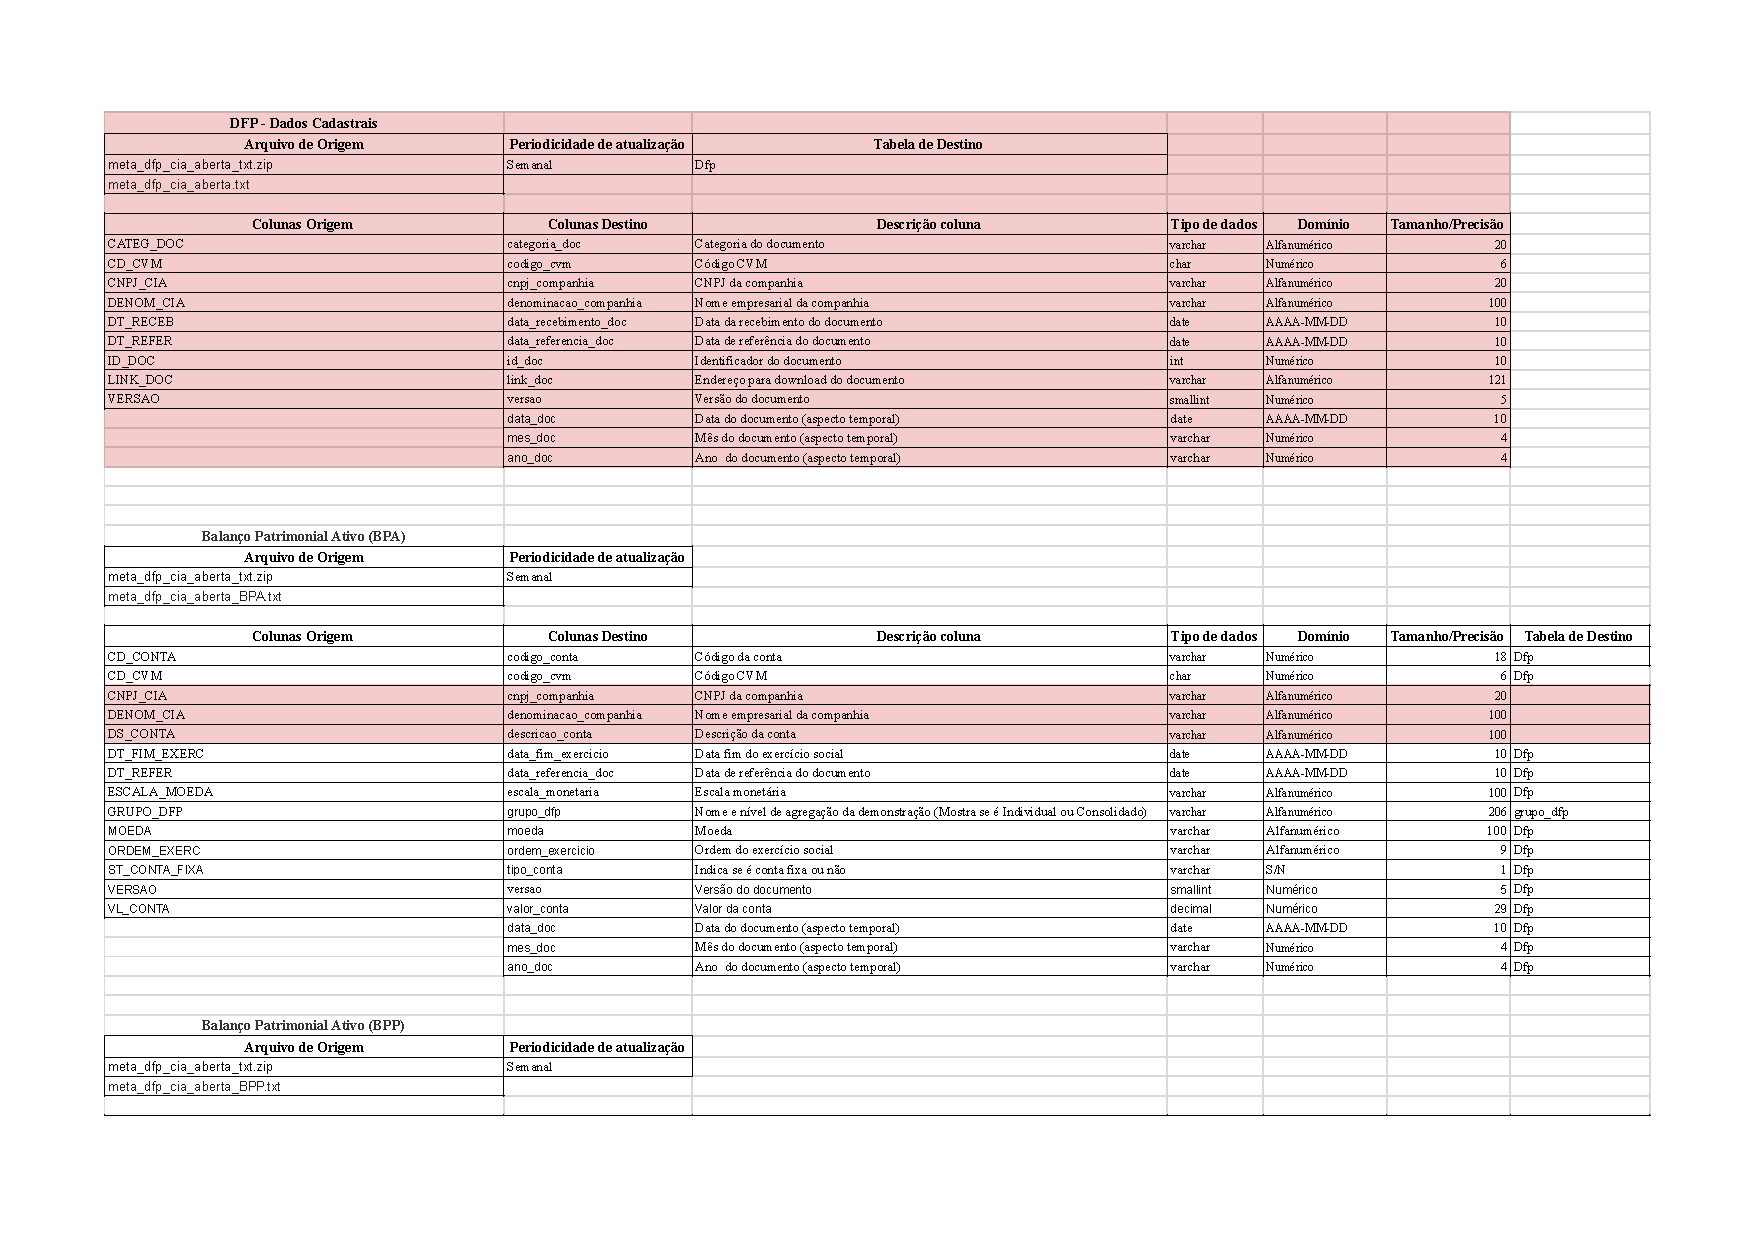
\includepdf[pages=-,frame=true]{apendice/Mapeamento CIA Aberta.pdf}
%
%
%\chapter{Código para baixar os dados da CVM}
%\label{ap:codigo-baixar}
%%\inputminted[linenos,frame=lines]{python}{codigo/baixar.py}
%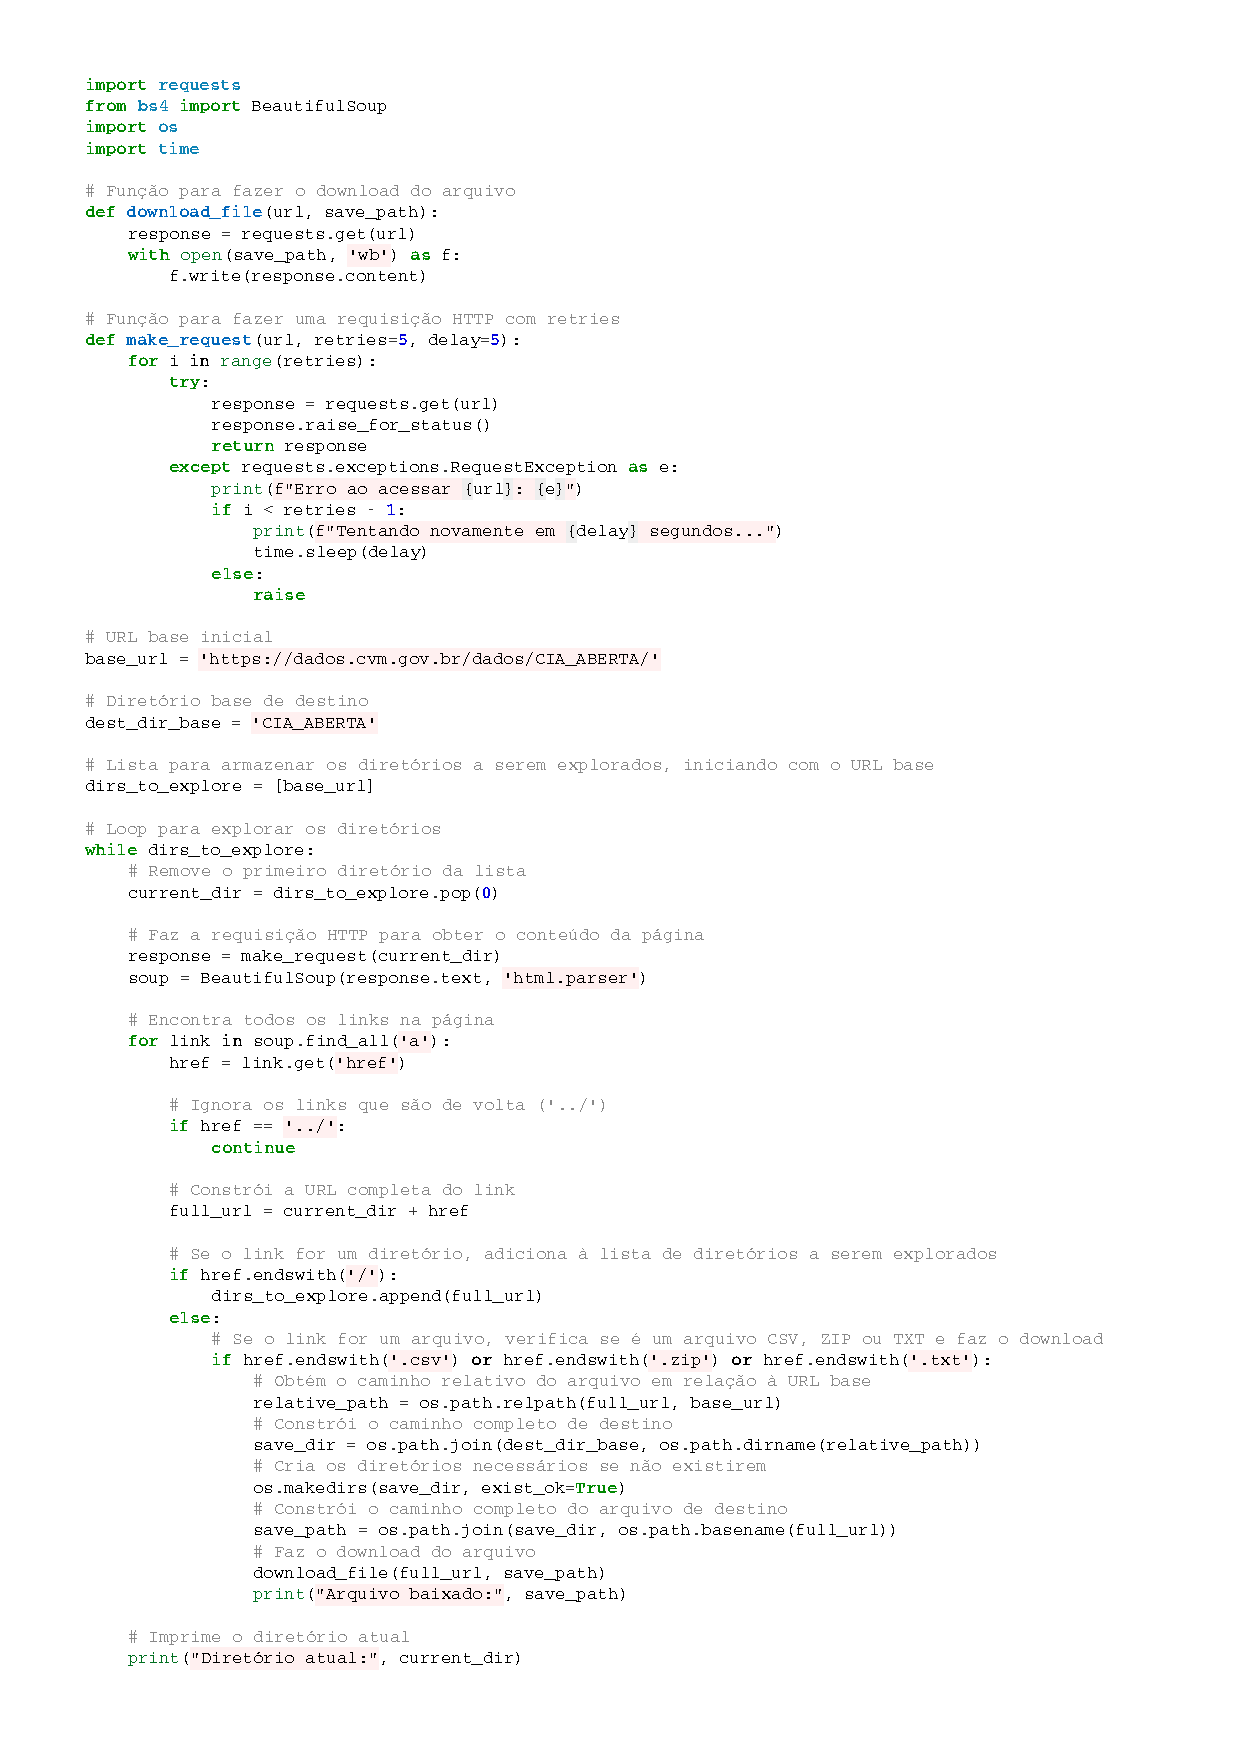
\includepdf[pages=-,frame=true]{codigo/baixar.pdf}
%
%\chapter{Código para extrair os dados da CVM}
%\label{ap:codigo-extrair}
%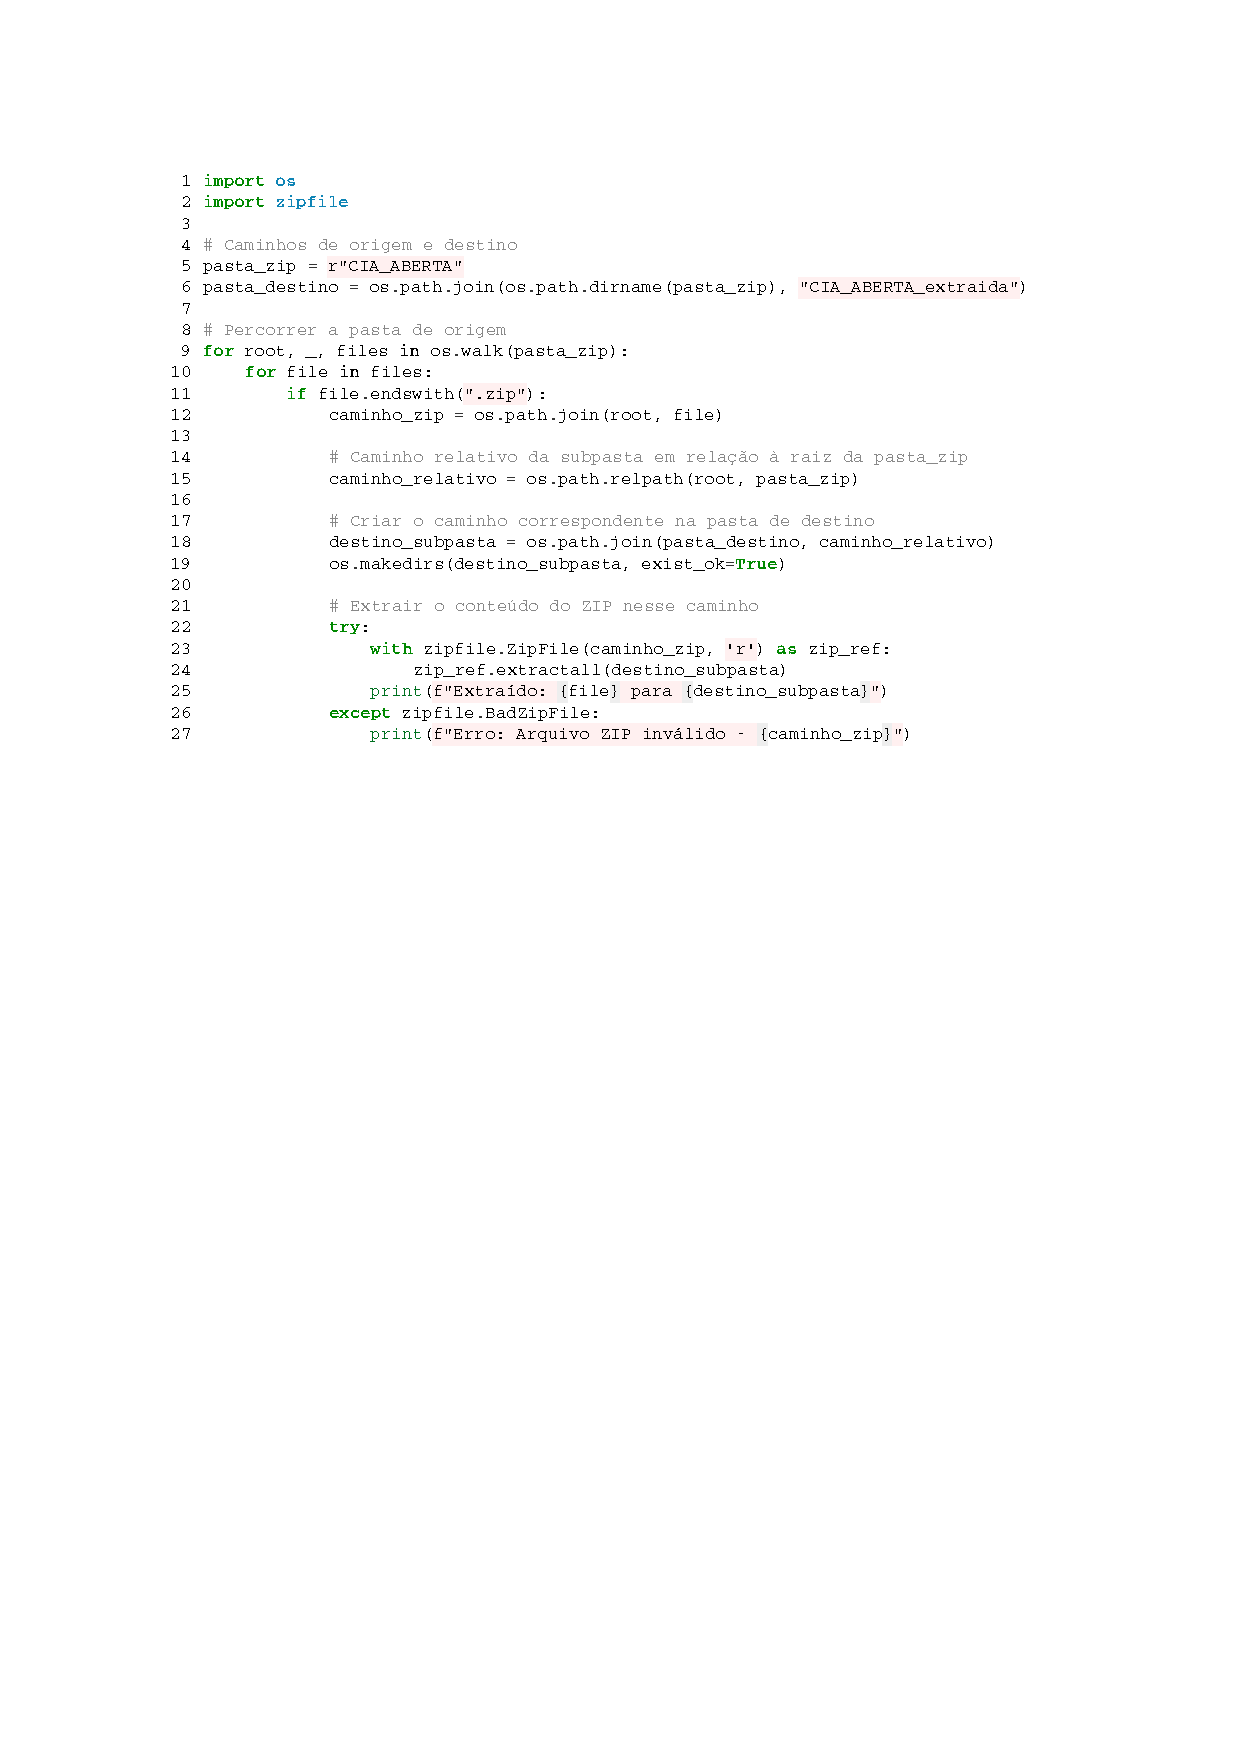
\includepdf[pages=-,frame=true]{codigo/extrair.pdf}


% Apêndices
\appendix
\renewcommand{\chaptername}{Apêndice}

\chapter{Código para baixar os dados da CVM}
\label{ap:codigo-baixar}
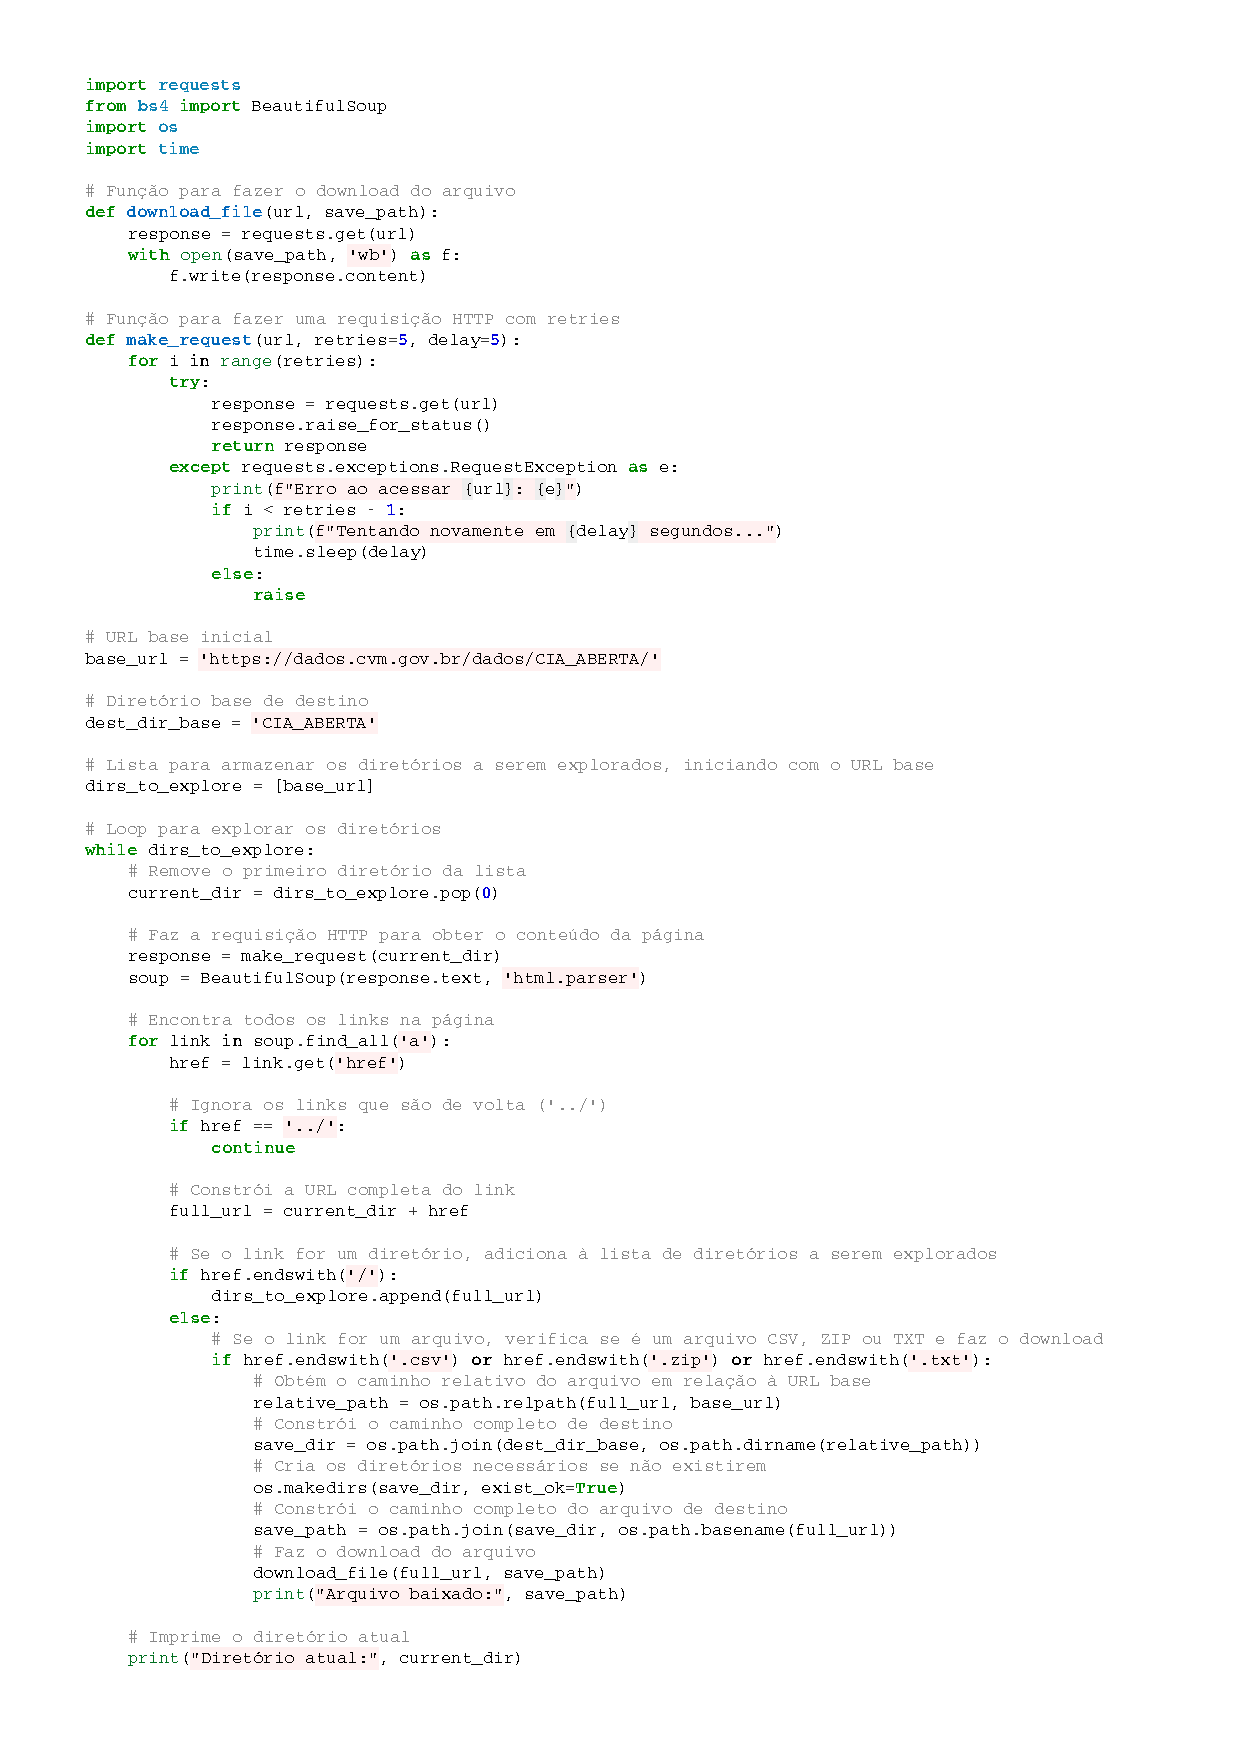
\includepdf[pages=-,frame=true]{codigo/baixar.pdf}

\chapter{Código para extrair os dados da CVM}
\label{ap:codigo-extrair}
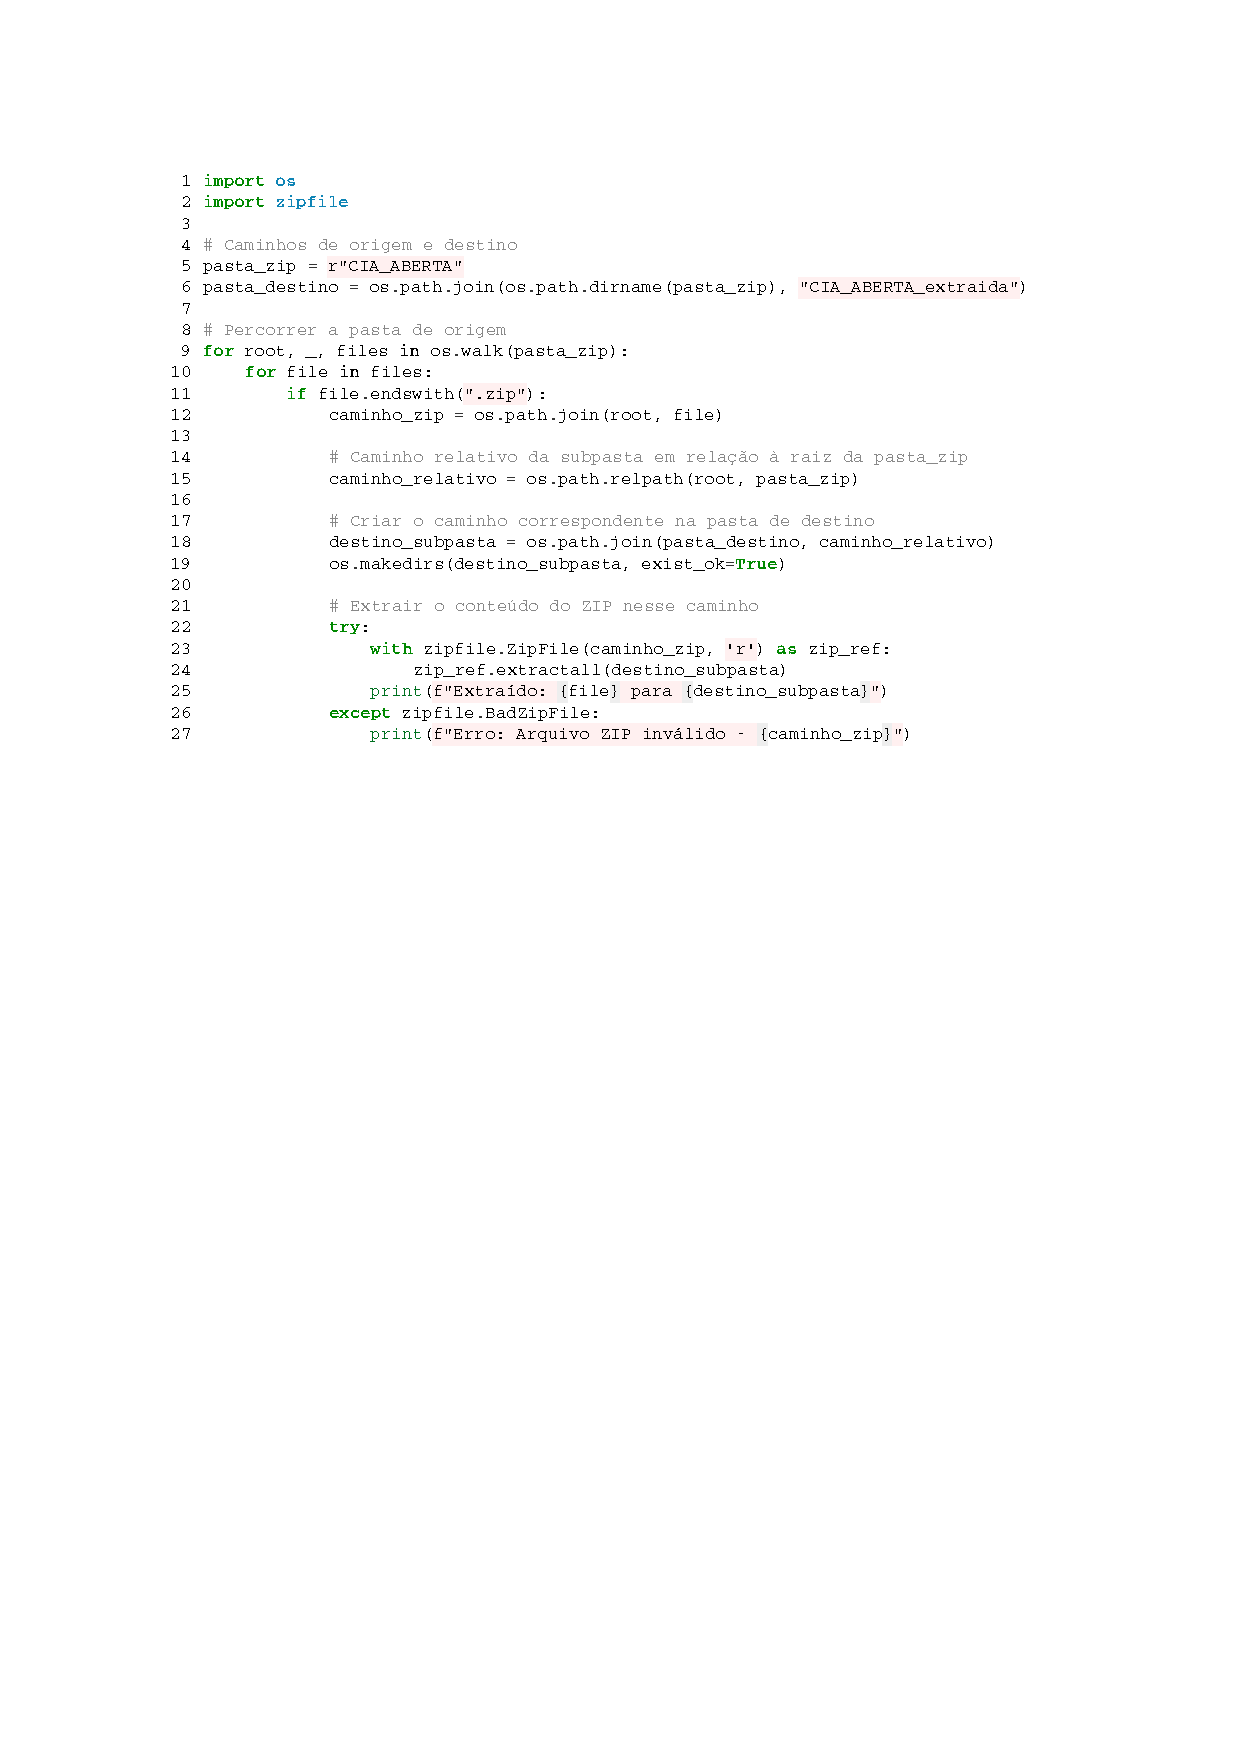
\includepdf[pages=-,frame=true]{codigo/extrair.pdf}

\chapter{Mapeamento Completo dos Dados da CVM}
\label{ap:mapeamento-cvm-dfp}
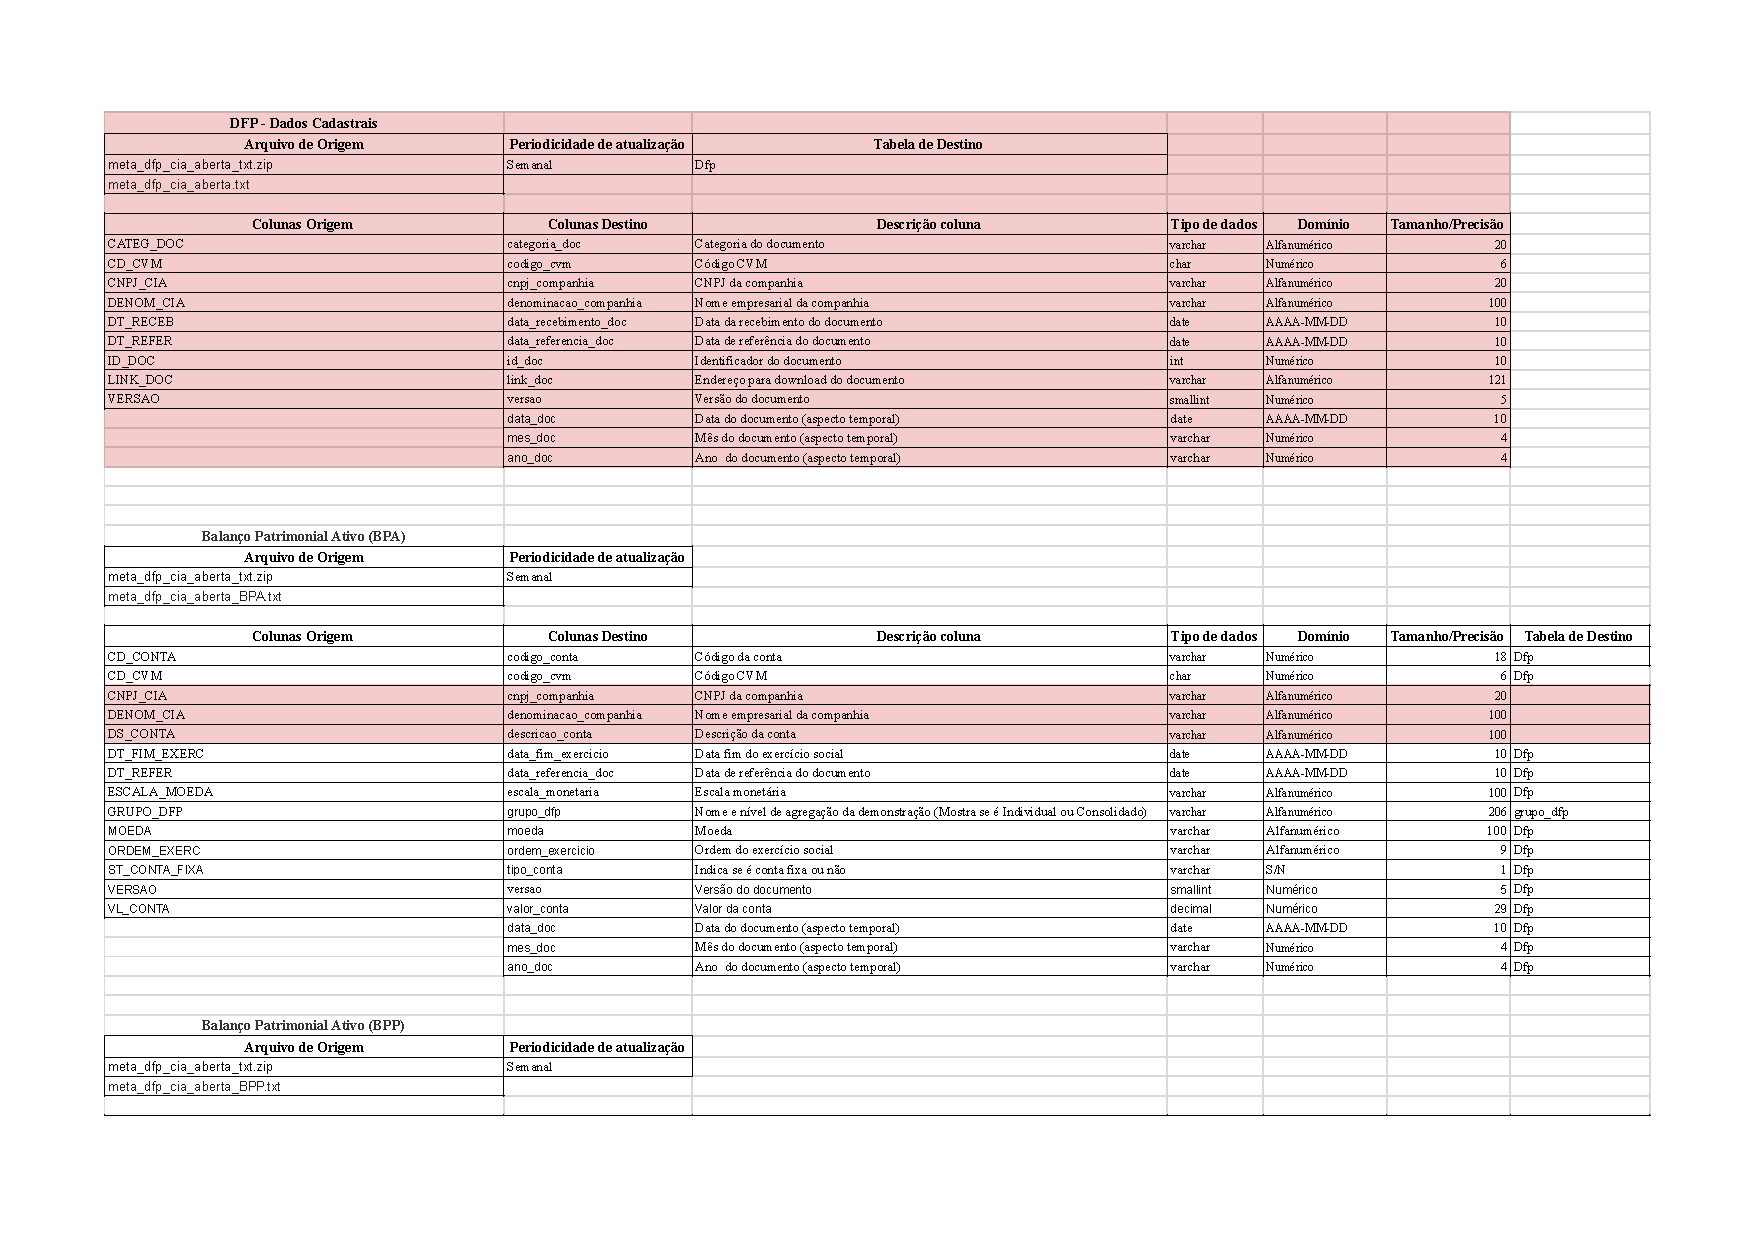
\includepdf[pages=-,frame=true]{apendice/Mapeamento CIA Aberta.pdf}


\chapter*{ÍNDICE}

\printindex

\end{document}
